% main.tex
% Fichero principal de transparencias (incluye a todos los demás).

% Compilar a .pdf con LaTeX (pdflatex)
% Es necesario instalar Beamer (paquete latex-beamer en Debian)
%

% Gráficos:
% Los gráficos pueden suministrarse en PNG, JPG, TIF, PDF, MPS
% Los EPS deben convertirse a PDF (usar epstopdf)
%
%\documentclass[17pt,aspectratio=169,hyperref={pdfusetitle,colorlinks,citecolor=blue,linkcolor=blue,urlcolor=blue}]{beamer}
\documentclass[17pt,aspectratio=169,hyperref={pdfusetitle,colorlinks,allcolors=olive}]{beamer}
\usetheme[orchid]{Hannover}
\beamertemplatenavigationsymbolsempty
\setbeamertemplate{headline}{}
\useoutertheme{infolines}

\usepackage{lmodern}
\usepackage[spanish]{babel}
\usepackage[utf8]{inputenc}
\usepackage{graphics}
\usepackage{multicol}
%\usepackage{amssymb} % Simbolos matematicos
%\usepackage[pdfusetitle]{hyperref}

%\usepackage{chronosys}

%% two slides per page
%\usepackage{pgfpages}
%\pgfpagesuselayout{2 on 1}[a4paper,border shrink=5mm]
%\usepackage{tikz}

\newcommand\YUGE{\fontsize{48}{60}\selectfont}

\newcommand{\secimage}{figs/bookpages}
\AtBeginSection[]
{
{
\usebackgroundtemplate{\includegraphics[width=\paperwidth,height=\paperheight]{\secimage}}
\begin{frame}<beamer>

  \begin{center}
    {\YUGE\bf\insertsection}
  \end{center}
\end{frame}

}
\renewcommand{\secimage}{figs/bookpages}
}

\title[Modelos Abiertos para IA Generativa]{Modelos Abiertos para Inteligencia Artificial Generativa}
%\subtitle{}
\author[Jesus M. Gonzalez-Barahona]{Jesus M. Gonzalez-Barahona}
\institute[URJC]{Universidad Rey Juan Carlos \
\url{https://floss.social/@jgbarah} ~~~~~ \url{https://jgbarah.github.io/presentations}}

\date[Mayo 2025]{\small Inteligencia Artificial: Actividades didácticas \\
Madrid, Spain, Mayo 19 2025~~~~~~~~
\includegraphics[width=1.2cm]{figs/by-sa}}

\begin{document}

%\begin{frame}[label=firstframe]
\begin{frame}
\maketitle
\end{frame}

%%-----------------------------------------
\begin{frame}

  \begin{center}
    Traducción realizada por \\
    Qwen/Qwen3-235B-A22B
  \end{center}
\end{frame}


%%-----------------------------------------
\begin{frame}
\frametitle{Plan}
%\begin{multicols}{2}
\tableofcontents
%\end{multicols}
\end{frame}

%%-----------------------------------------
%%-----------------------------------------
%\section{¿Qué es el ``aprendizaje automático''?}

%%-----------------------------------------
% \begin{frame}[fragile]
% \frametitle{¡Empieza probando!}

% \begin{center}
% 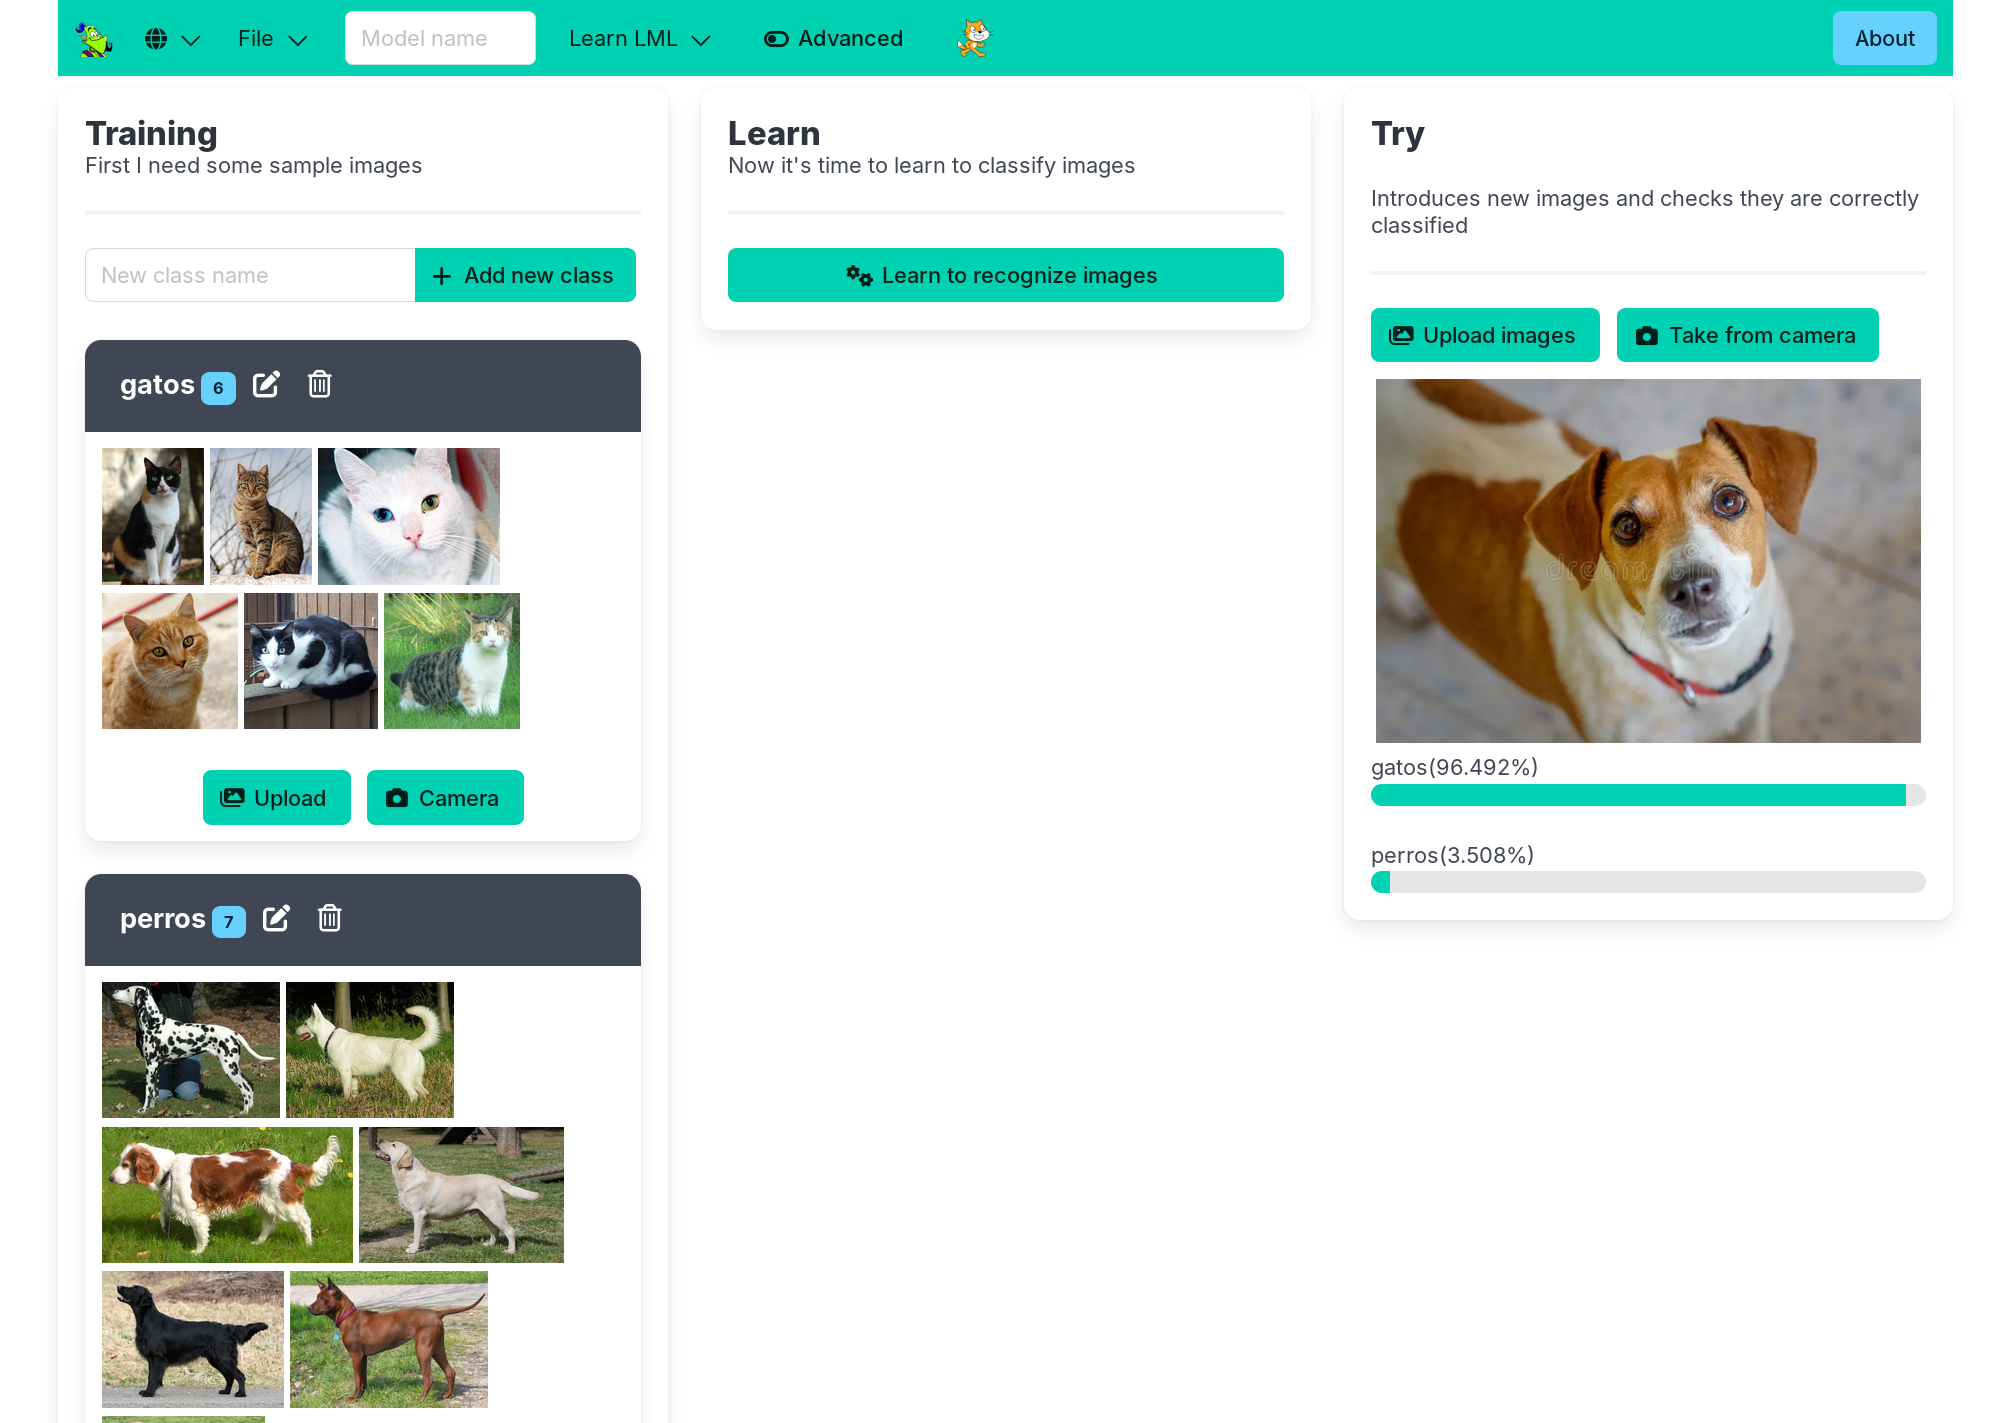
\includegraphics[width=9cm]{figs/learningml}
% \end{center}
% \end{frame}

% %% -----------------------------------------
% \begin{frame}[fragile]
% \frametitle{¡Empieza probando!}

% \begin{center}
% {\Large
% \url{https://v2.learningml.org/}
% }
% \end{center}
% \end{frame}

%%-----------------------------------------
%%-----------------------------------------
\section{¿Qué es un modelo ``abierto''?}

%%-----------------------------------------
\begin{frame}[fragile]
\frametitle{¡Empieza probando!}

\begin{center}
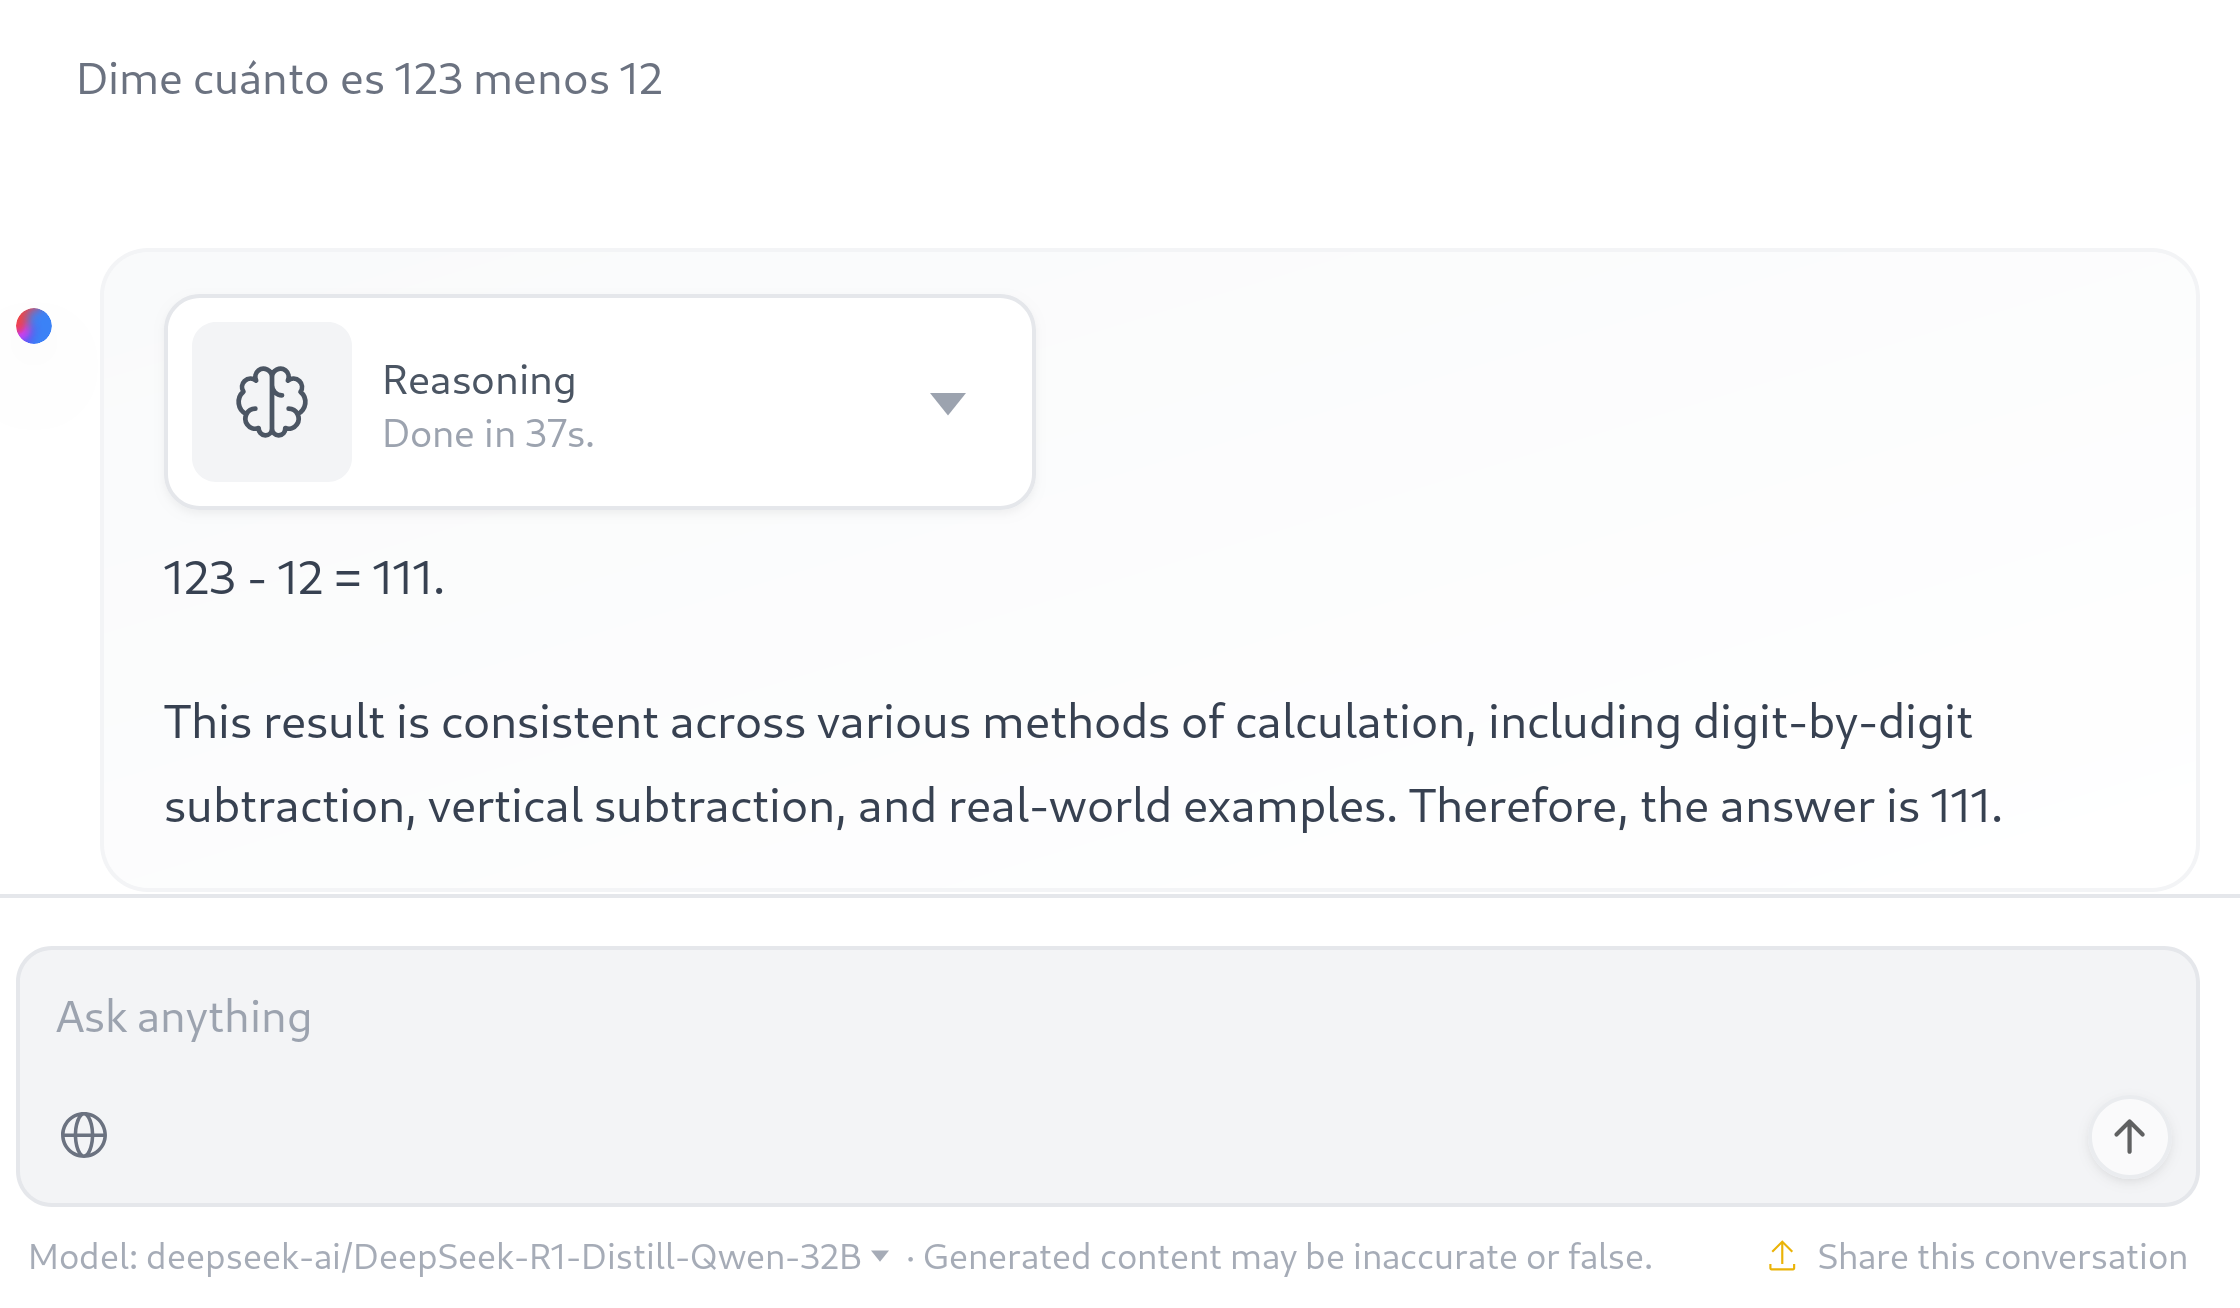
\includegraphics[width=9cm]{figs/huggingchat-deepseek}
\end{center}
\end{frame}

%%-----------------------------------------
\begin{frame}[fragile]
\frametitle{¡Empieza probando!}

\begin{center}
{\large
\url{https://huggingface.co/chat/}
}
\end{center}
\end{frame}

%%-----------------------------------------
\begin{frame}[fragile]
\frametitle{Modelos para texto, imágenes...}

\begin{columns}[T]
\begin{column}{.58\textwidth}
    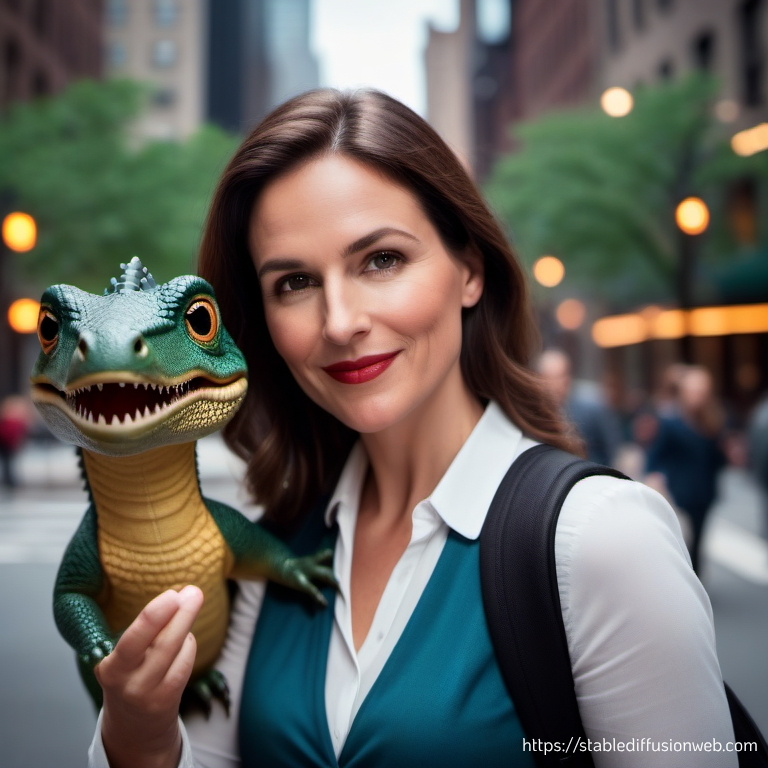
\includegraphics[width=7cm]{figs/selfie}
\end{column}%
\hfill%
\begin{column}{.38\textwidth}
  {\small Stable Diffusion XL:} \\
  selfie de un profesor con un dinosaurio, en Manhattan \\
  cinematic-default \\
\end{column}%

\end{columns}

\end{frame}

%%-----------------------------------------
\begin{frame}[fragile]
\frametitle{¡Pero ojo!}

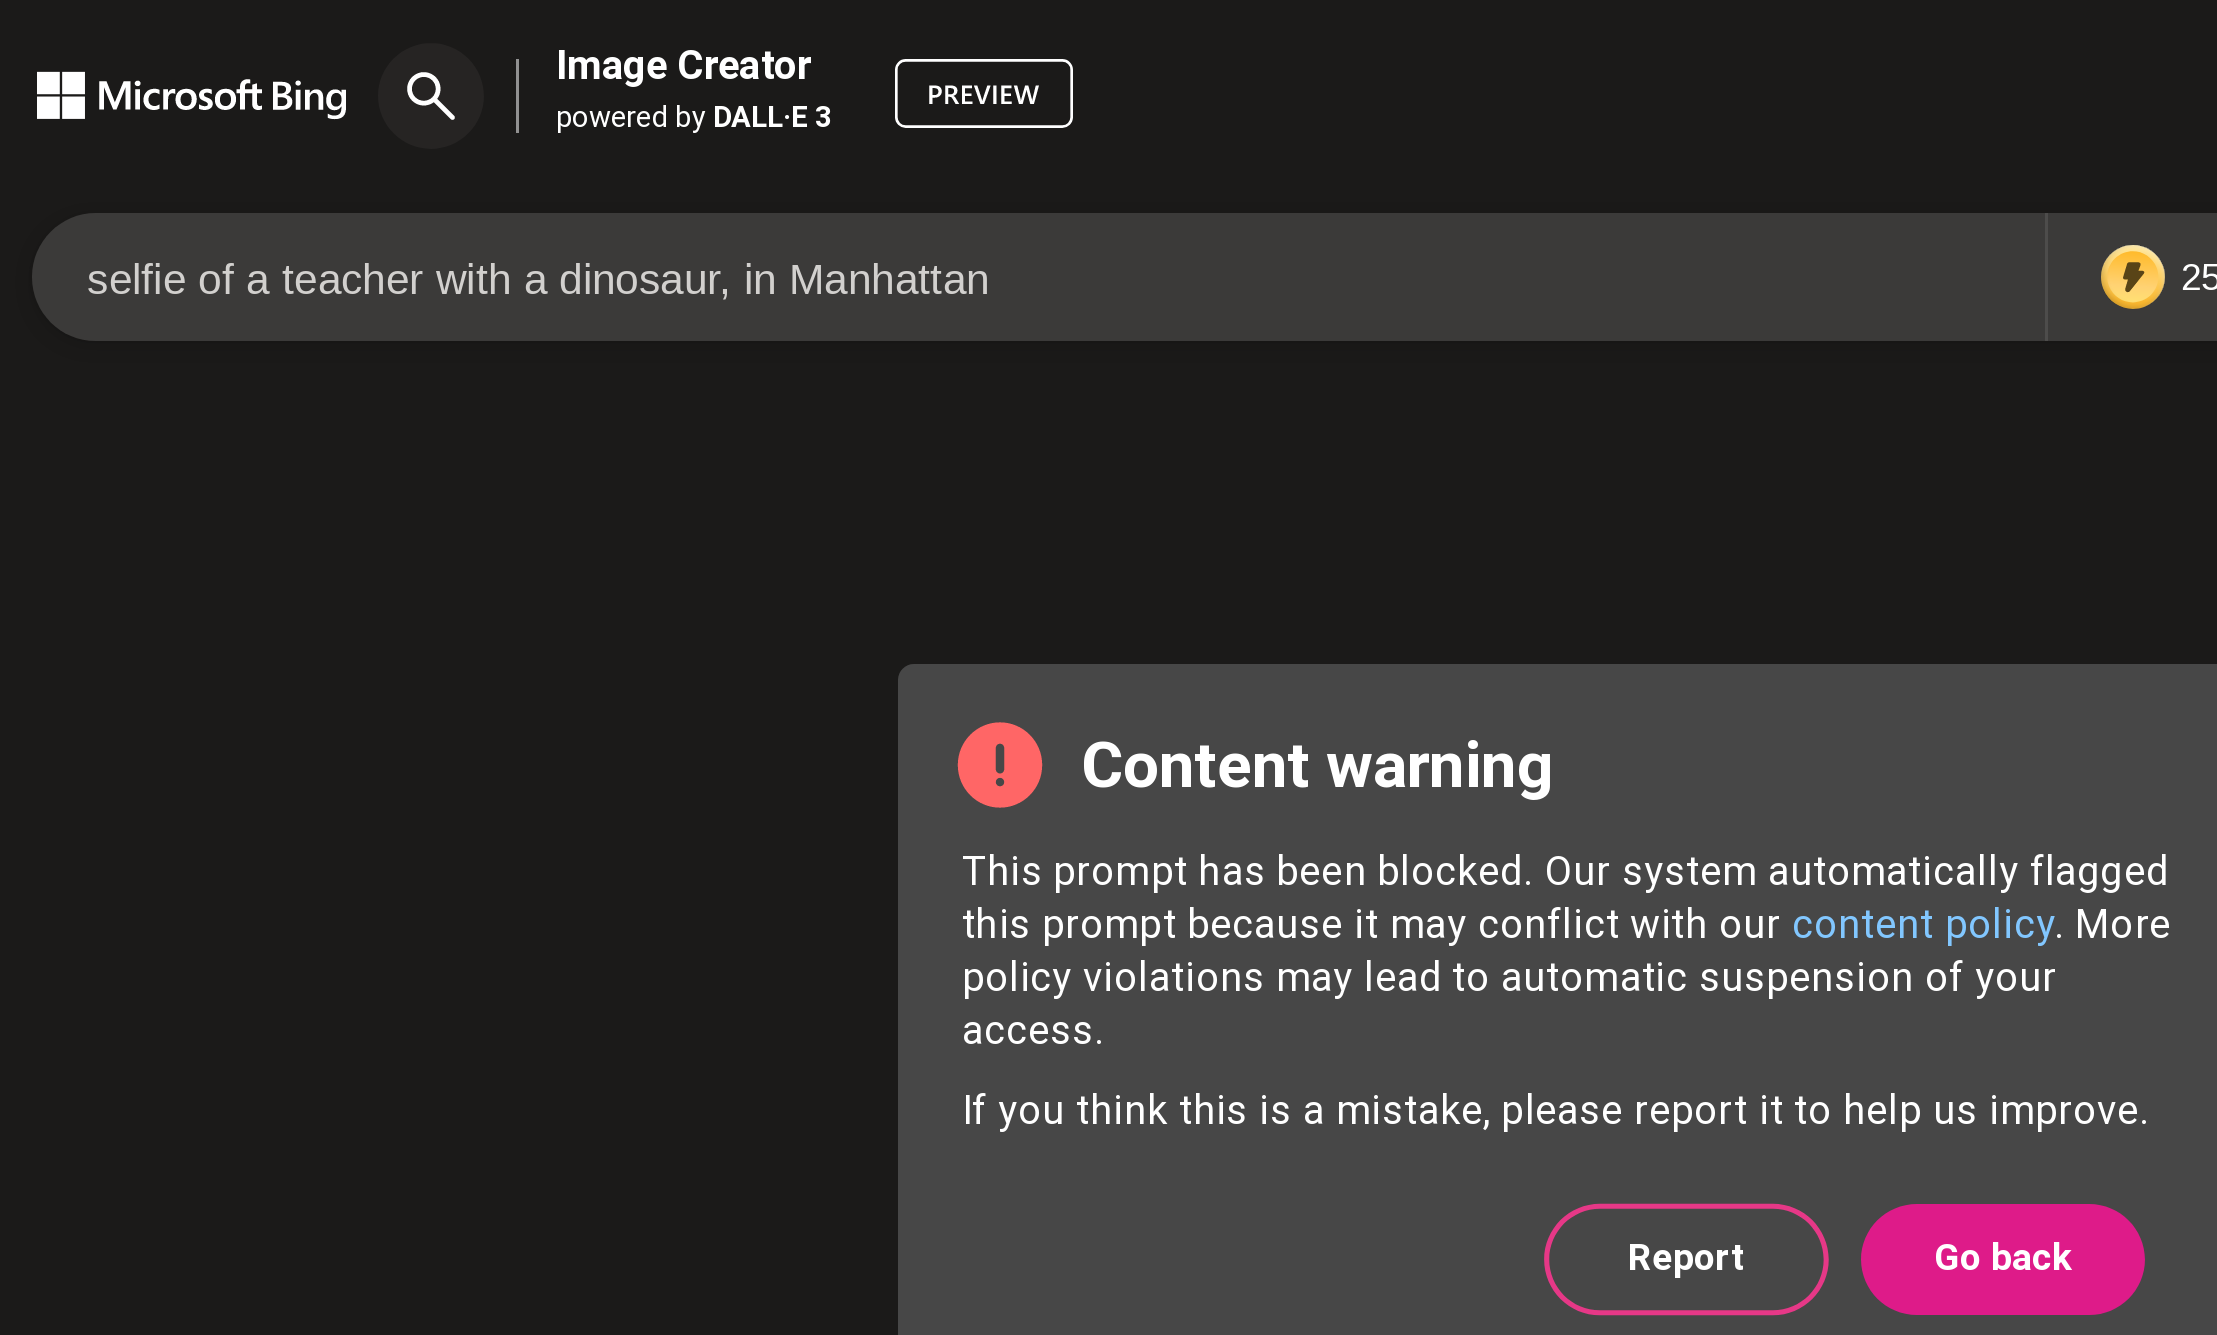
\includegraphics[width=6.5cm]{figs/bing-content-warning}

{\small
``selfie de un profesor con un dinosaurio, en Manhattan''
}
\end{frame}

%%-----------------------------------------
\begin{frame}[fragile]

{\Large
¿Podemos controlar \\
cómo usamos \\
los modelos generativos? \\
}
\end{frame}

%%-----------------------------------------
\begin{frame}[fragile]
\frametitle{¿Qué es un modelo generativo?}

\begin{itemize}
\item Arquitectura
\item Pesos, solo pesos
\item Software para inferencia
\end{itemize}

Pero también:

\begin{itemize}
\item Datos para entrenamiento y benchmark
\item Software para entrenamiento y benchmark
\item Pesos de modelos intermedios
\item Documentación, explicando todo
\end{itemize}
\end{frame}

%% -----------------------------------------
\begin{frame}[fragile]
\frametitle{Ejemplo: Stable Diffusion}

  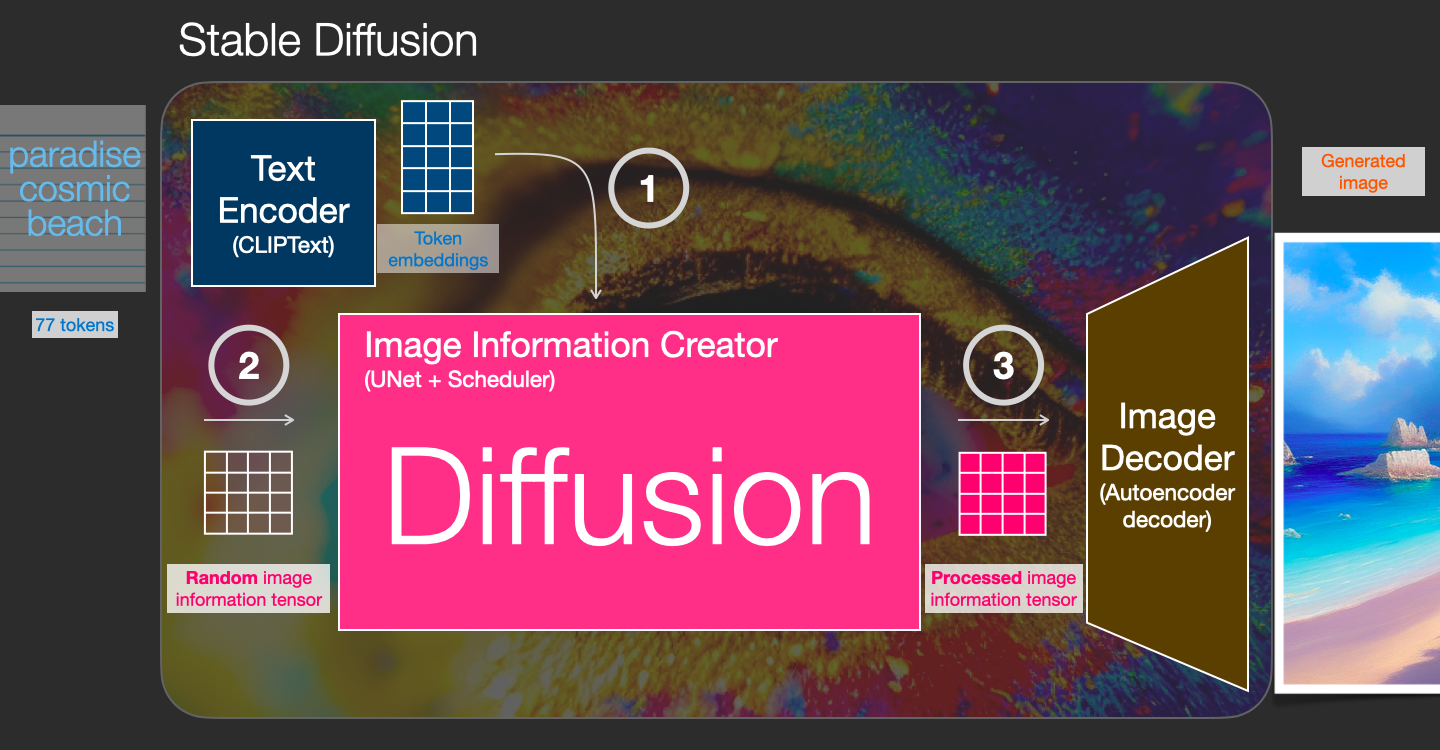
\includegraphics[width=10cm]{figs/sd-process}

\begin{flushright}
{\scriptsize
\url{https://jalammar.github.io/illustrated-stable-diffusion/}
}
\end{flushright}

\end{frame}

%%-----------------------------------------
\begin{frame}[fragile]
\frametitle{}

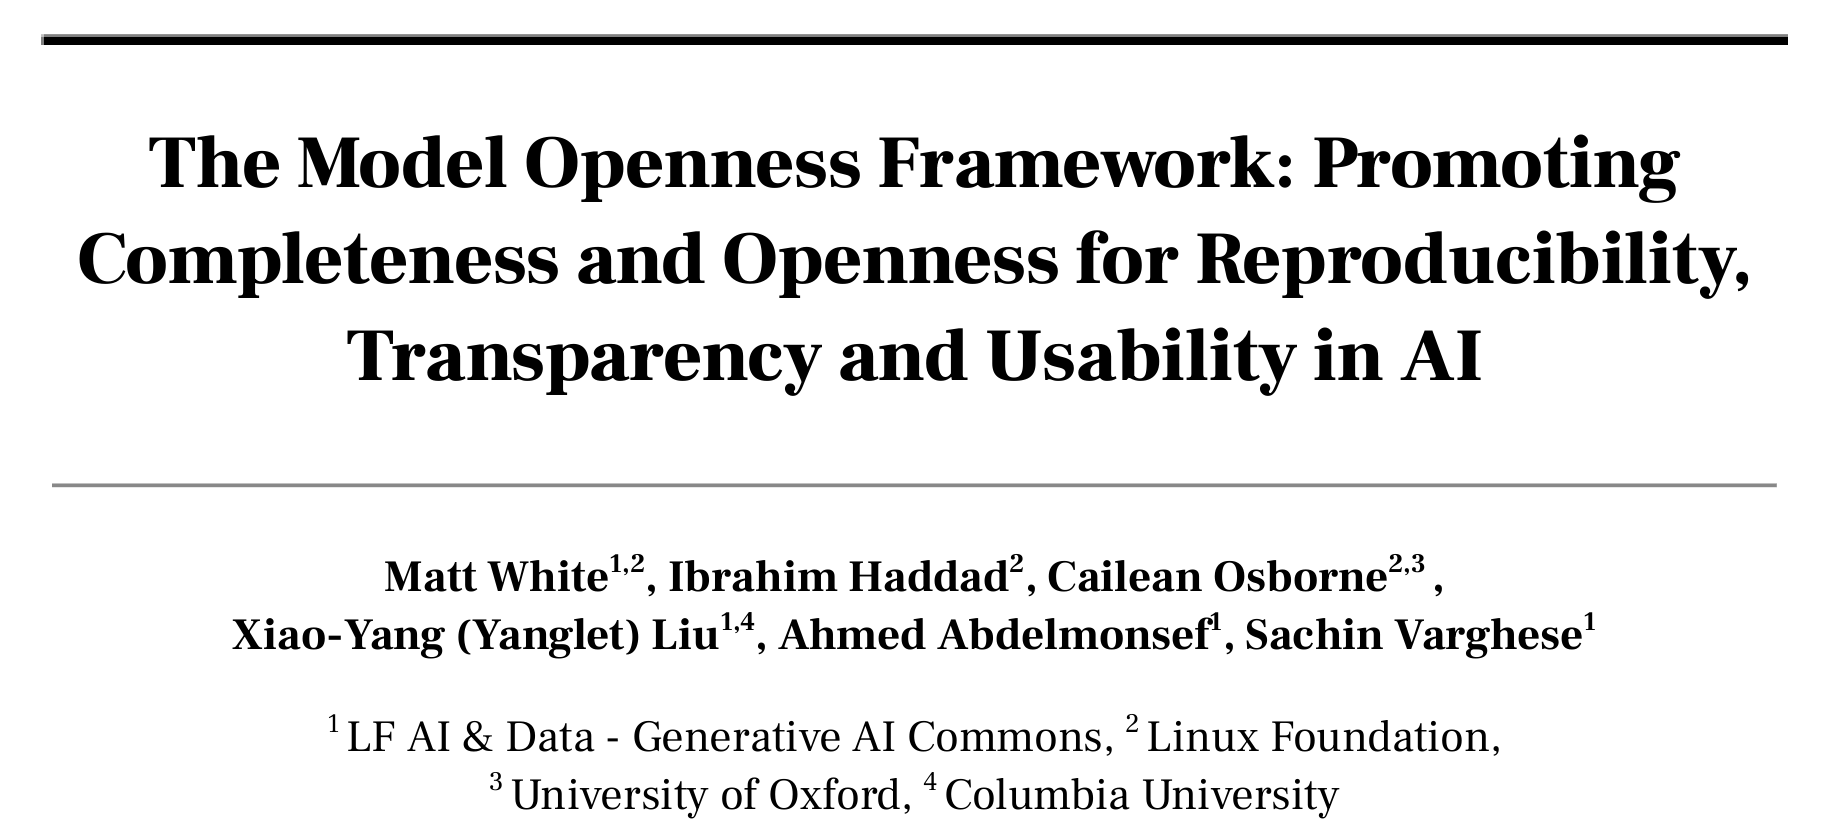
\includegraphics[height=6cm]{figs/paper-openess-framework}

\begin{flushright}
{\small
\url{https://arxiv.org/abs/2403.13784}
}
\end{flushright}

\end{frame}

%%-----------------------------------------
\begin{frame}[fragile]
\frametitle{Clases de ``apertura''}

\begin{itemize}
\item Ciencia abierta: artículo, conjuntos de datos, archivos de registro, parámetros y metadatos de modelos intermedios
\item Herramientas abiertas: código para entrenamiento, inferencia y evaluación, bibliotecas, datos de evaluación
\item Modelo abierto: arquitectura, parámetros y metadatos del modelo, informe técnico, tarjeta del modelo, tarjeta de datos
\end{itemize}

\end{frame}

%%-----------------------------------------
\begin{frame}[fragile]
\frametitle{``Modelo reproductible abierto''}

Todo lo anterior, y

\begin{center}
{\Large conjunto completo de entrenamiento}
\end{center}

(y cualquier otro detalle necesario para producir el mismo modelo binario)
\end{frame}

%%-----------------------------------------
\begin{frame}[fragile]
\frametitle{Para cada uno...}

\begin{itemize}
\item Libertad de uso
\item Libertad de estudio
\item Libertad de modificación
\item Libertad de compartir
\end{itemize}
\end{frame}

%%-----------------------------------------
\begin{frame}[fragile]
\frametitle{Mínimo para ejecutar en tu computadora}

\begin{itemize}
\item Código de inferencia, con bibliotecas
\item Arquitectura del modelo
\item Parámetros y metadatos del modelo (pesos)
\item Informe técnico (prompts, etc.)
\item Tarjeta del modelo (opcional)
\end{itemize}

\end{frame}

%%-----------------------------------------
\begin{frame}[fragile]
\frametitle{Requisitos de equipo}

\begin{itemize}
\item Depende de la arquitectura y el tamaño del modelo
\item La CPU puede ser suficiente, la GPU acelera mucho
\item RAM suficiente para que quepa el modelo
\item El código suele ser software libre
\end{itemize}

\end{frame}

%%-----------------------------------------
\begin{frame}[fragile]
\frametitle{Ejemplo: HuggingChat}

\begin{center}
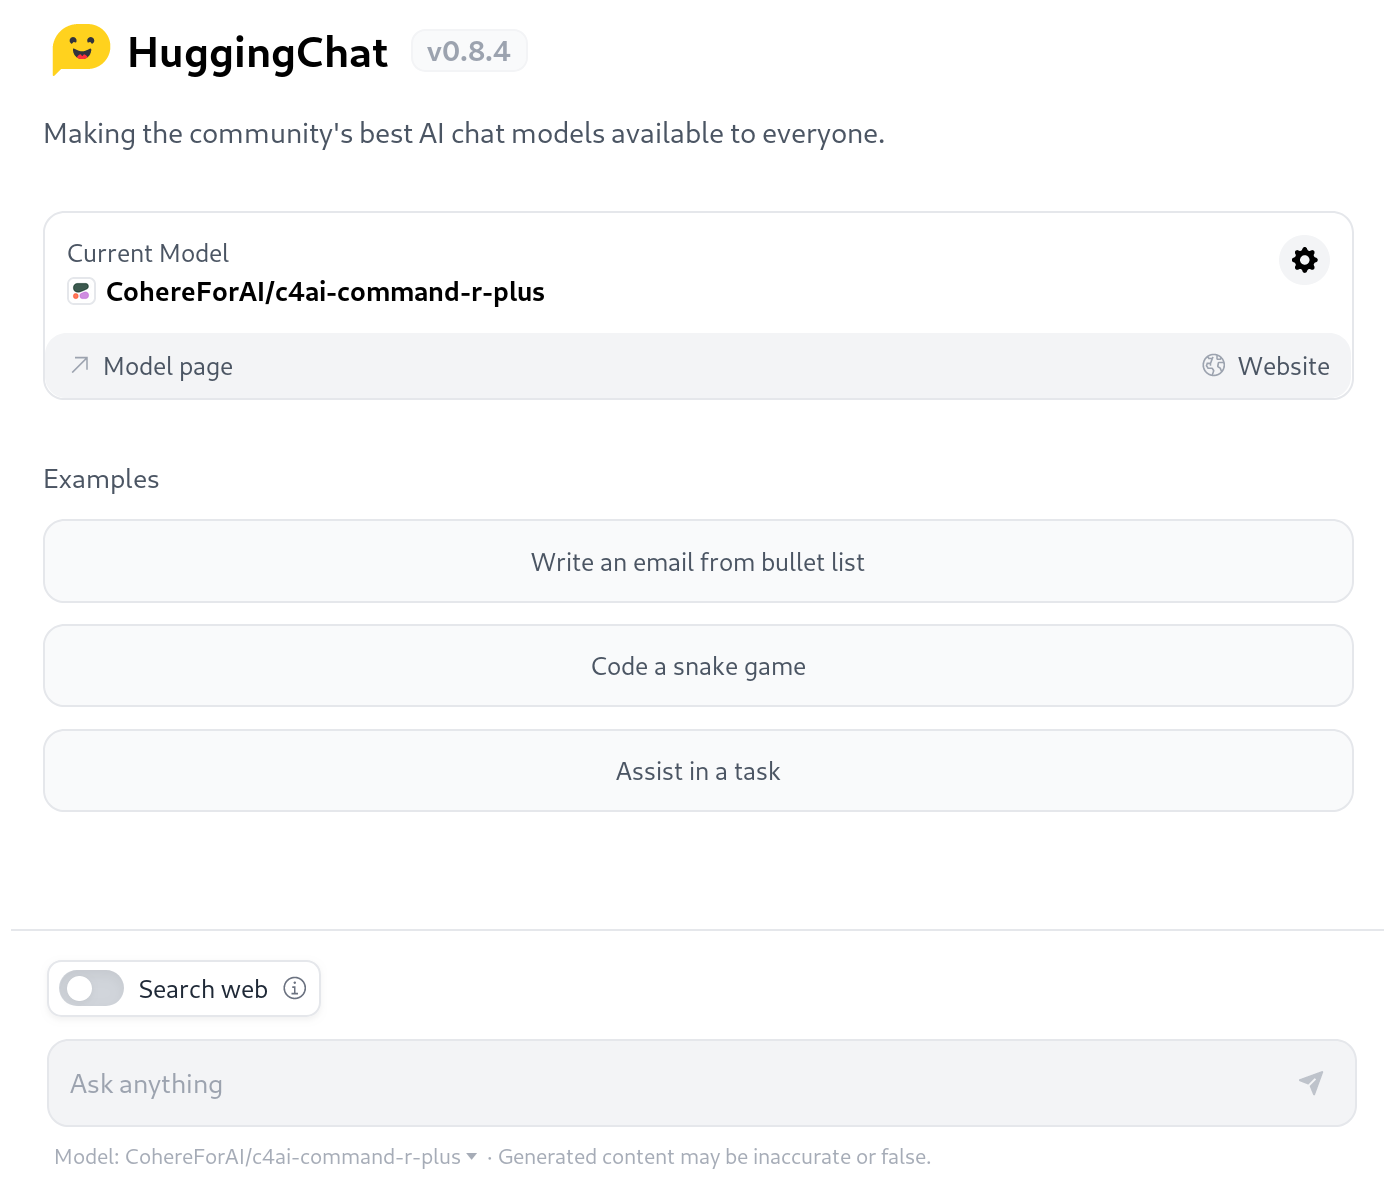
\includegraphics[width=6cm]{figs/huggingchat}
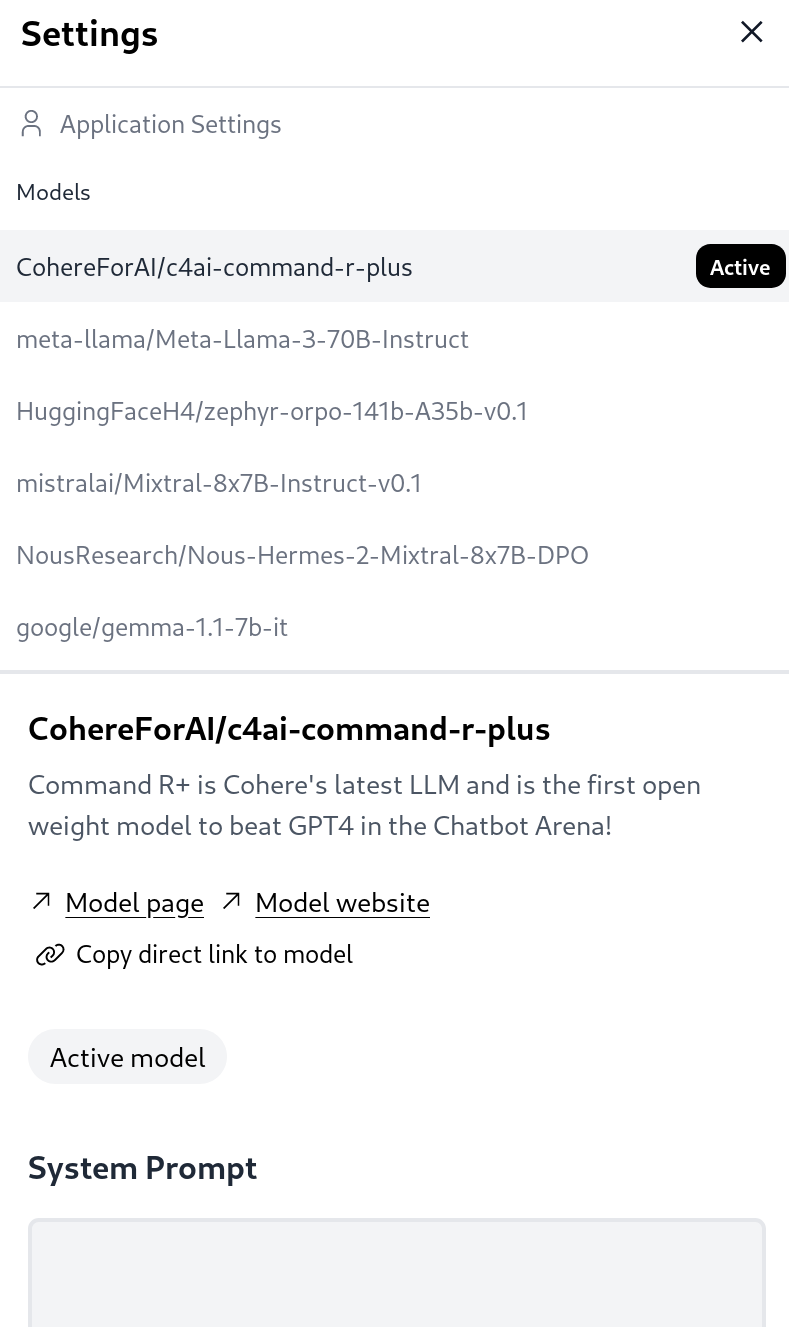
\includegraphics[width=3cm]{figs/huggingchat-models}
\end{center}

\begin{flushright}
{\small
\url{https://huggingface.co/chat/}
}
\end{flushright}
\end{frame}

%%-----------------------------------------
\begin{frame}[fragile]
\frametitle{Ejemplo: computer-agent}

\begin{center}
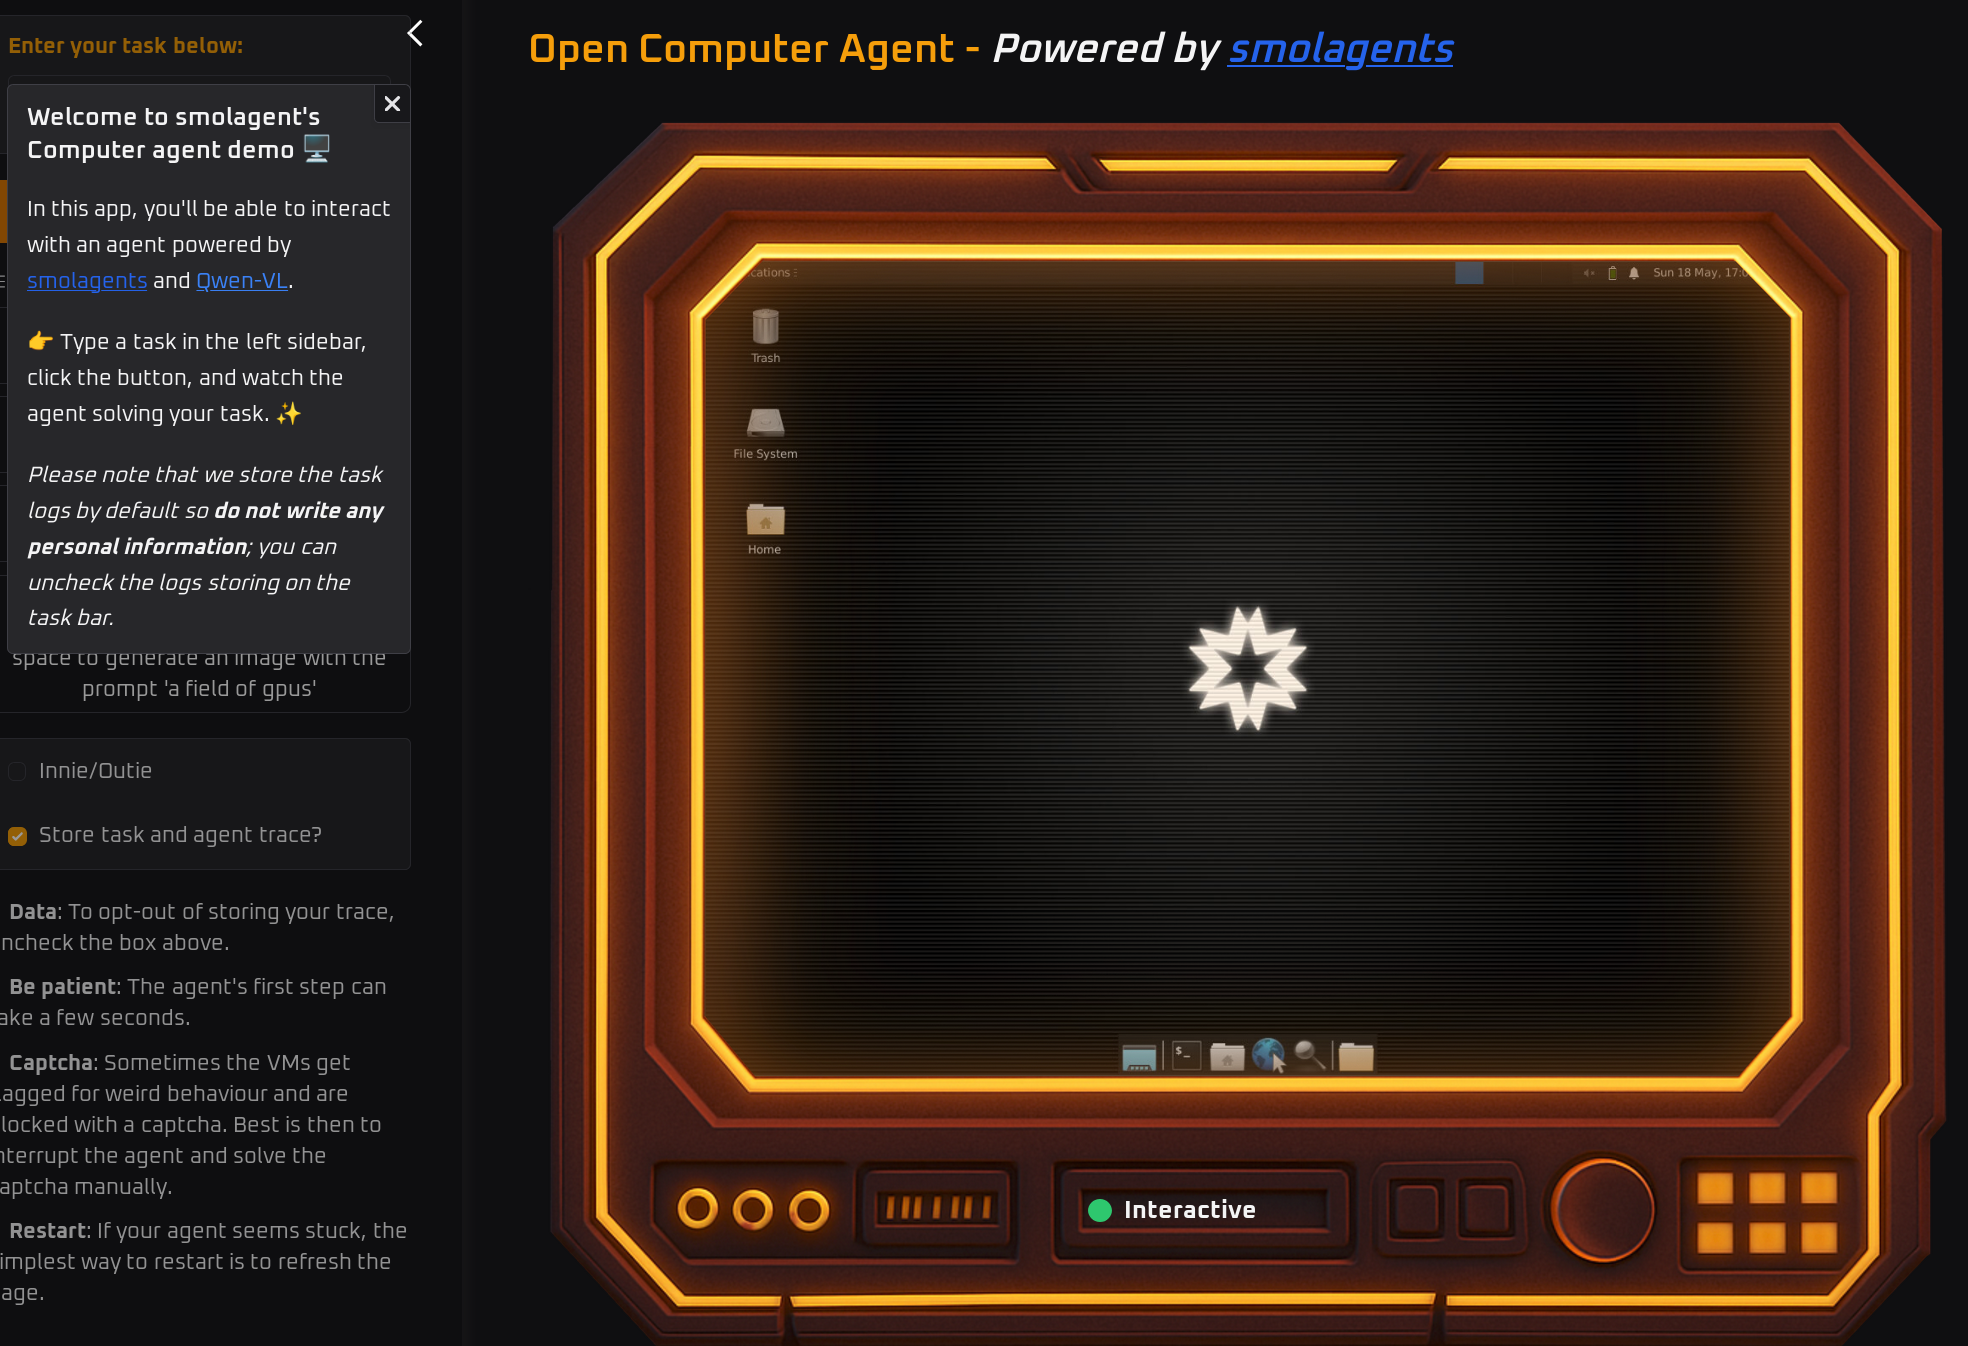
\includegraphics[width=7.5cm]{figs/computer-agent}
\end{center}

\begin{flushright}
{\footnotesize
\url{https://huggingface.co/spaces/smolagents/computer-agent}
}
\end{flushright}
\end{frame}

%%-----------------------------------------
\begin{frame}[fragile]
\frametitle{Ejemplo: computer-agent}

Componentes clave:

\begin{itemize}
\item Marco de agentes: smolagents
\item Modelo: Qwen2-VL-72B
\item Escritorio: E2B Desktop
\end{itemize}

\begin{flushright}
{\footnotesize
\url{https://github.com/huggingface/smolagents} \\
\url{https://huggingface.co/Qwen/Qwen2-VL-72B-Instruct} \\
\url{https://github.com/e2b-dev/desktop} \\
}
\end{flushright}
\end{frame}

%%-----------------------------------------
\begin{frame}[fragile]
\frametitle{Ejemplo: DreamO}

\begin{center}
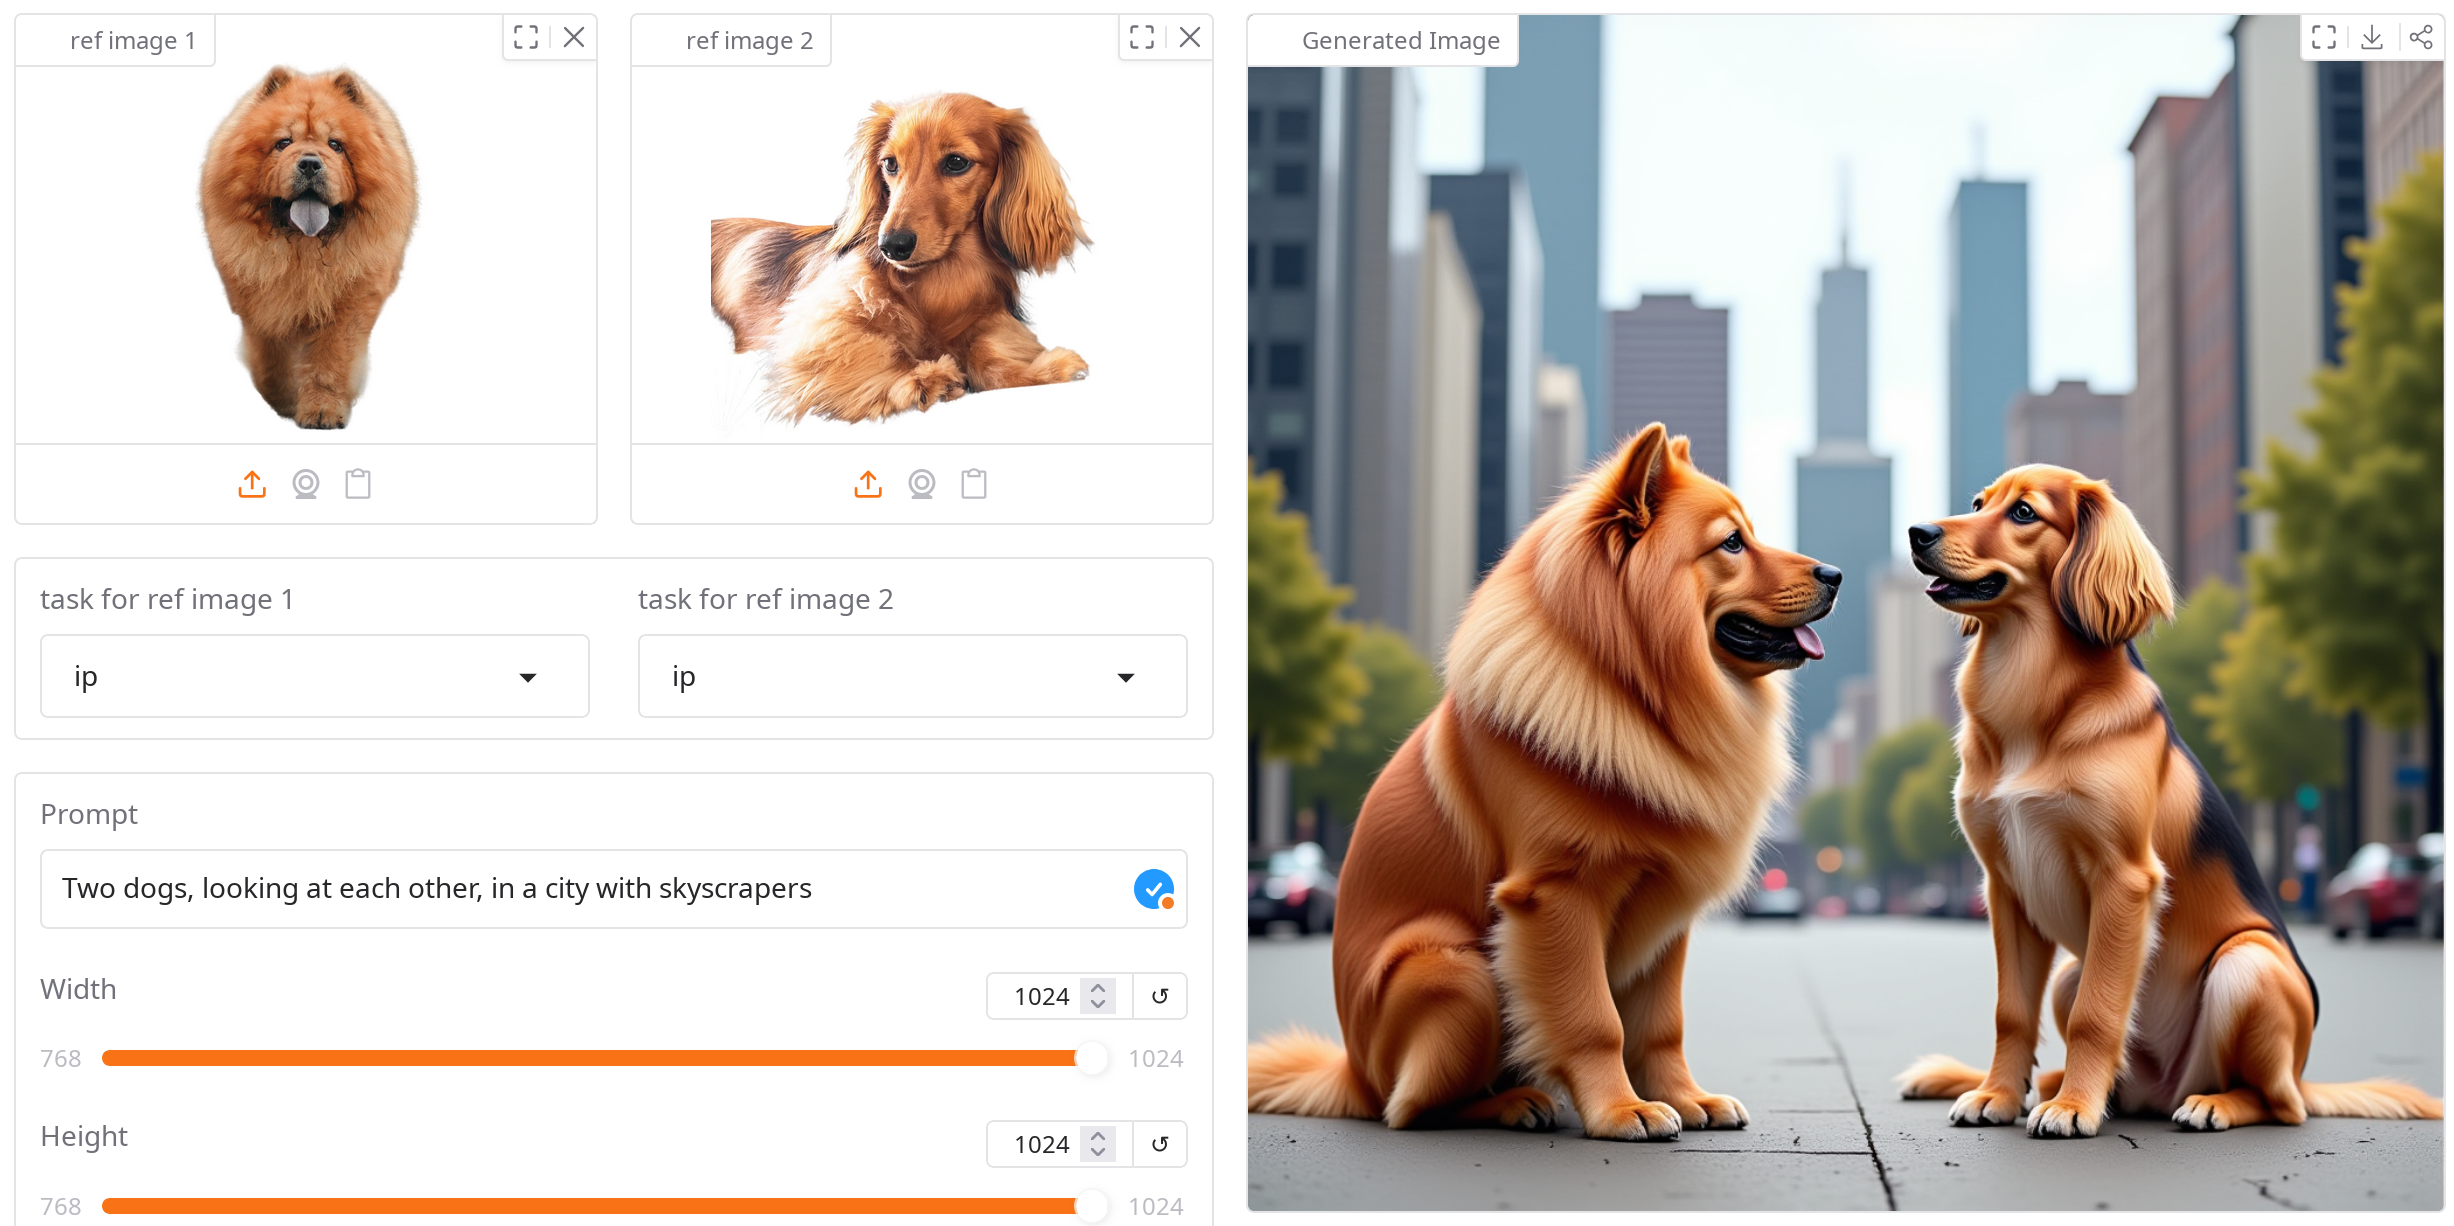
\includegraphics[width=10cm]{figs/dreamo}
\end{center}

\begin{flushright}
{\small
\url{https://huggingface.co/spaces/ByteDance/DreamO}
}
\end{flushright}
\end{frame}

%%-----------------------------------------
\begin{frame}[fragile]
\frametitle{Ejemplo: DeepSite}

\begin{center}
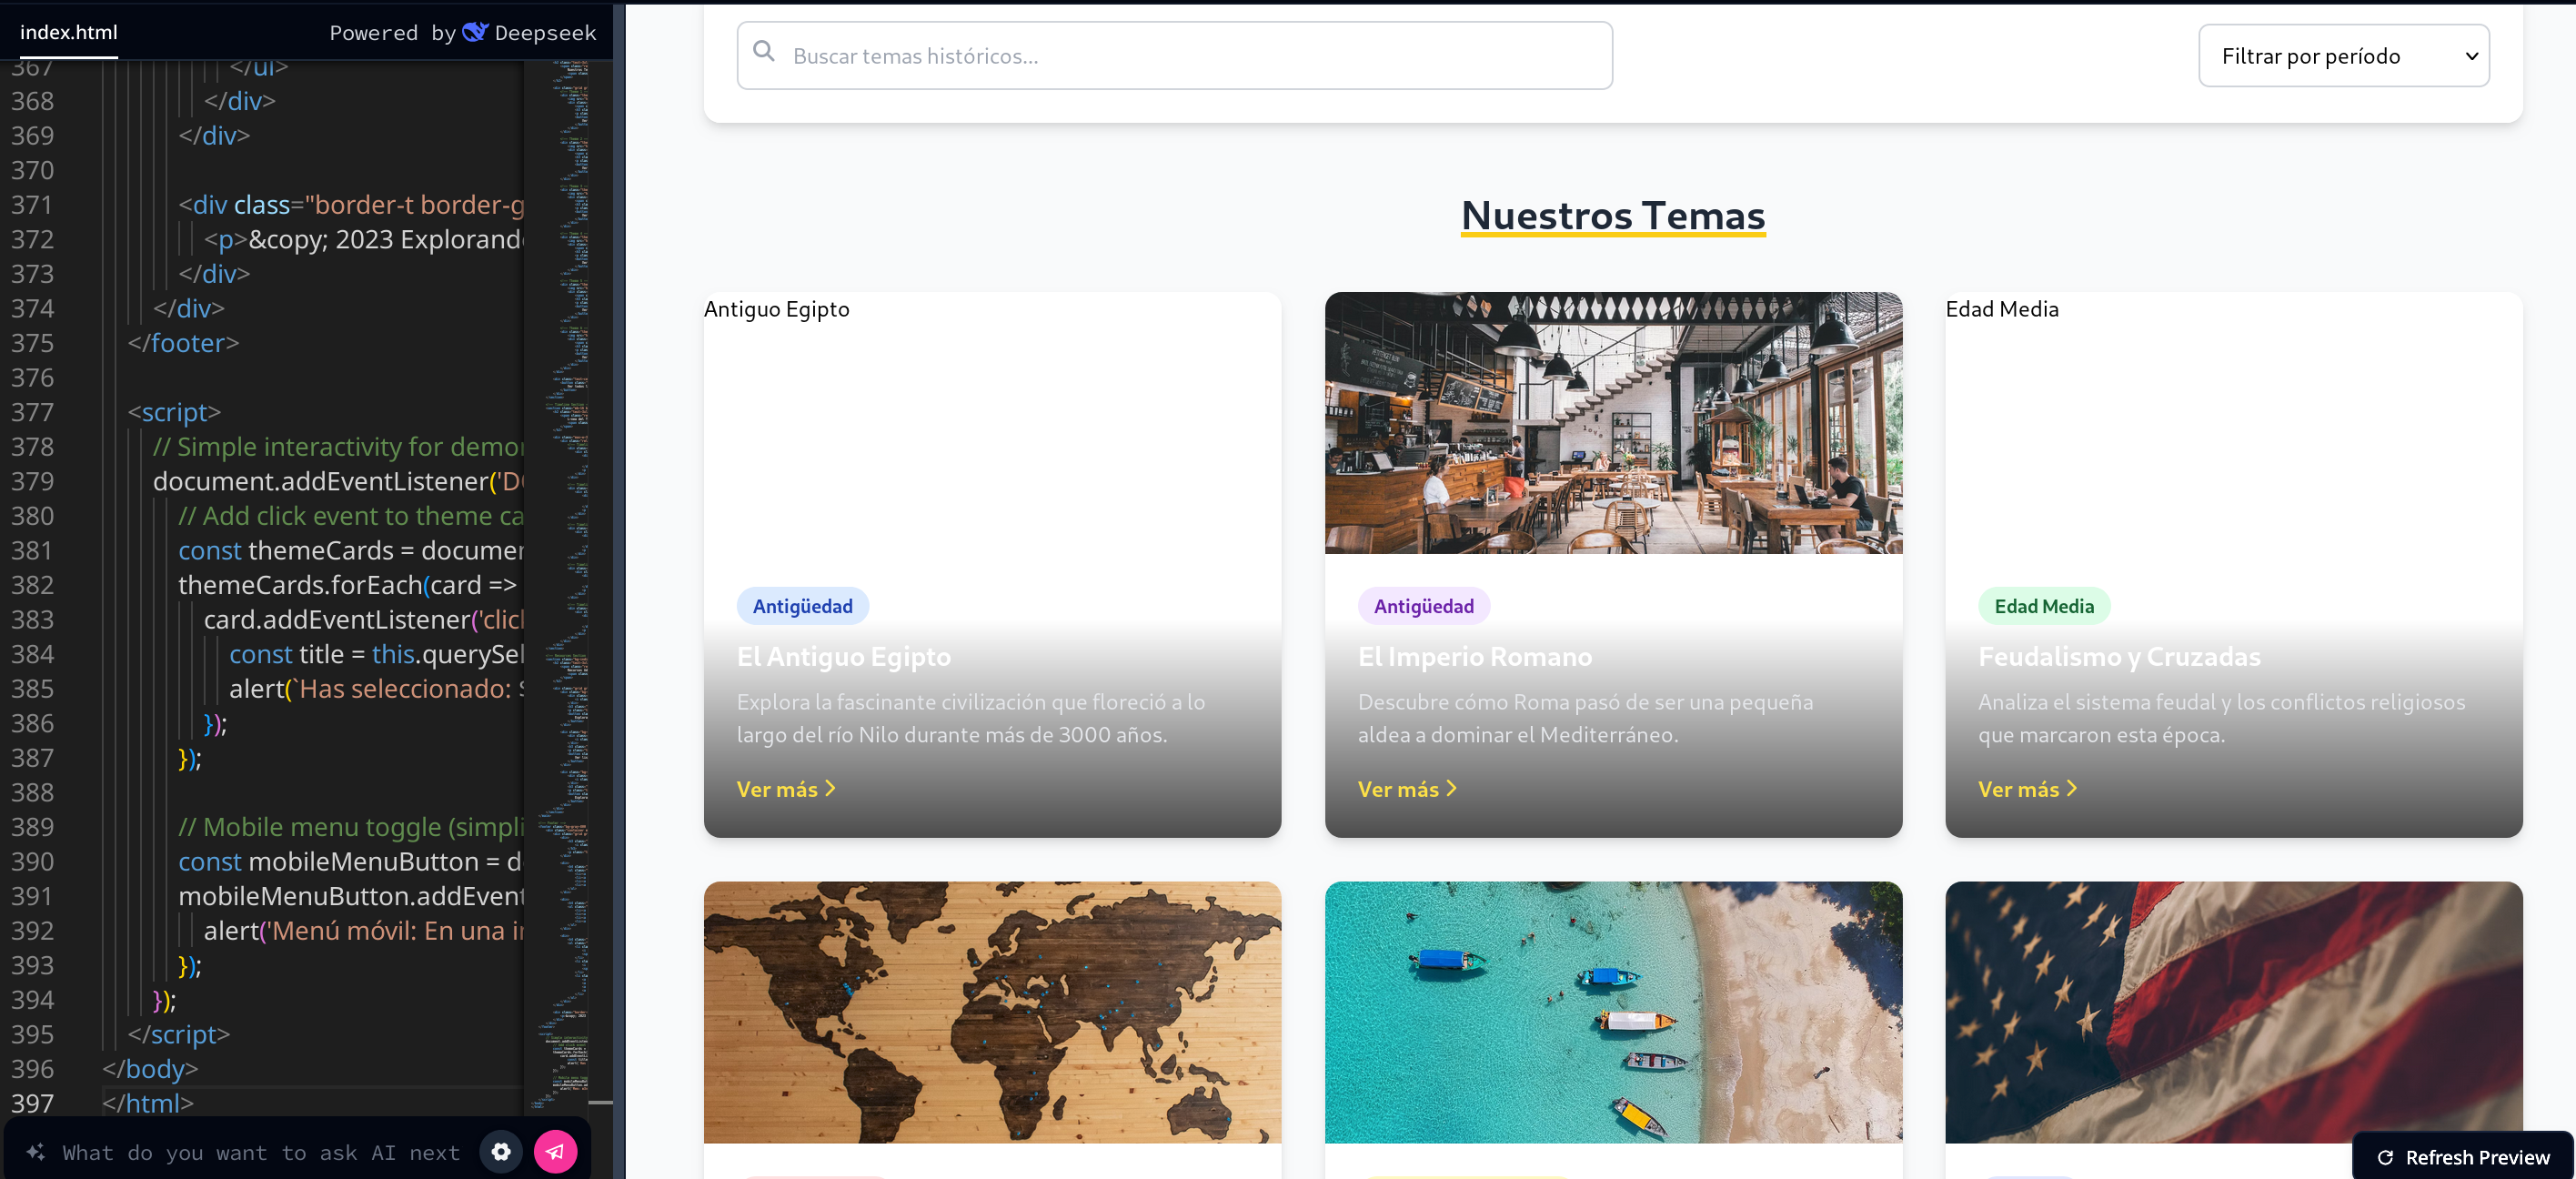
\includegraphics[width=10.5cm]{figs/deepsite}
\end{center}

\begin{flushright}
{\scriptsize
\url{https://huggingface.co/spaces/enzostvs/deepsite} \\
\url{https://huggingface.co/spaces/enzostvs/deepsite/discussions/74}
}
\end{flushright}
\end{frame}

%%-----------------------------------------
\begin{frame}[fragile]
\frametitle{Más ejemplos}

\begin{flushright}
{
\url{https://huggingface.co/spaces/}
}
\end{flushright}
\end{frame}

%%-----------------------------------------
%%-----------------------------------------
\section{IA generativa en tu computadora}

%%-----------------------------------------
\begin{frame}[fragile]
\frametitle{Voz a texto: Whisper}

% 
\includegraphics[width=8.5cm]{figs/whisper}
{\small
\begin{verbatim}
#!/usr/bin/python3
import whisper

model = whisper.load_model('tiny')
transcription = model.transcribe('recording.wav')
print(transcription['text'])
\end{verbatim}
}

\begin{verbatim}
$ whisper speech.wav --language Spanish
\end{verbatim}

\begin{flushright}
{\scriptsize
\url{https://openai.com/blog/whisper/} \\
\url{https://github.com/openai/whisper} \\
Licencia: MIT (código abierto) \\
}
\end{flushright}

\end{frame}

%%-----------------------------------------
\begin{frame}[fragile]
\frametitle{Texto a voz: Coqui TTS}

{\small
\begin{verbatim}
$ tts --text "Texto"
--model_name tts_models/es/mai/tacotron2-DDC
--out_path speech.wav
\end{verbatim}
}

\begin{flushright}
{\small
\url{https://github.com/idiap/coqui-ai-TTS} \\
Licencia: MPL-2.0 (código abierto) \\
}
\end{flushright}

\end{frame}

%% -----------------------------------------
\begin{frame}[fragile]
\frametitle{Stable Diffusion}

EasyDiffusion:
\begin{flushright}
\url{https://easydiffusion.github.io}
\end{flushright}

Fooocus:
\begin{flushright}
\url{https://github.com/lllyasviel/Fooocus}
\end{flushright}

AUTOMATIC1111:
\begin{flushright}
\url{https://github.com/AUTOMATIC1111/stable-diffusion-webui}
\end{flushright}

\end{frame}

%% -----------------------------------------
\begin{frame}[fragile]
\frametitle{Stable Diffusion (2)}

SD.next:
\begin{flushright}
\url{https://github.com/vladmandic/automatic}
\end{flushright}

ComfyUI:
\begin{flushright}
\url{https://github.com/comfyanonymous/ComfyUI}
\end{flushright}

\end{frame}

%% -----------------------------------------
\begin{frame}[fragile]
\frametitle{Modelos de generación de texto}

Llama4, Licencia de la Comunidad Llama
\begin{flushright}
\url{https://llama.com/models/llama-4/} \\
\url{https://github.com/meta-llama/}
\end{flushright}

DeepSeek, Licencia DeepSeek

\begin{flushright}
\url{https://deepseek.com/}
\url{https://huggingface.co/deepseek-ai}
\end{flushright}

\end{frame}

%% -----------------------------------------
\begin{frame}[fragile]
\frametitle{Modelos de generación de texto (2)}

Mistral, Apache 2.0

\begin{flushright}
\url{https://mistral.ai/}
\url{https://huggingface.co/mistralai}
\end{flushright}

Qwen, Apache 2.0

\begin{flushright}
\url{https://huggingface.co/Qwen}
\end{flushright}

\end{frame}

%% -----------------------------------------
\begin{frame}[fragile]
\frametitle{Clasificación}

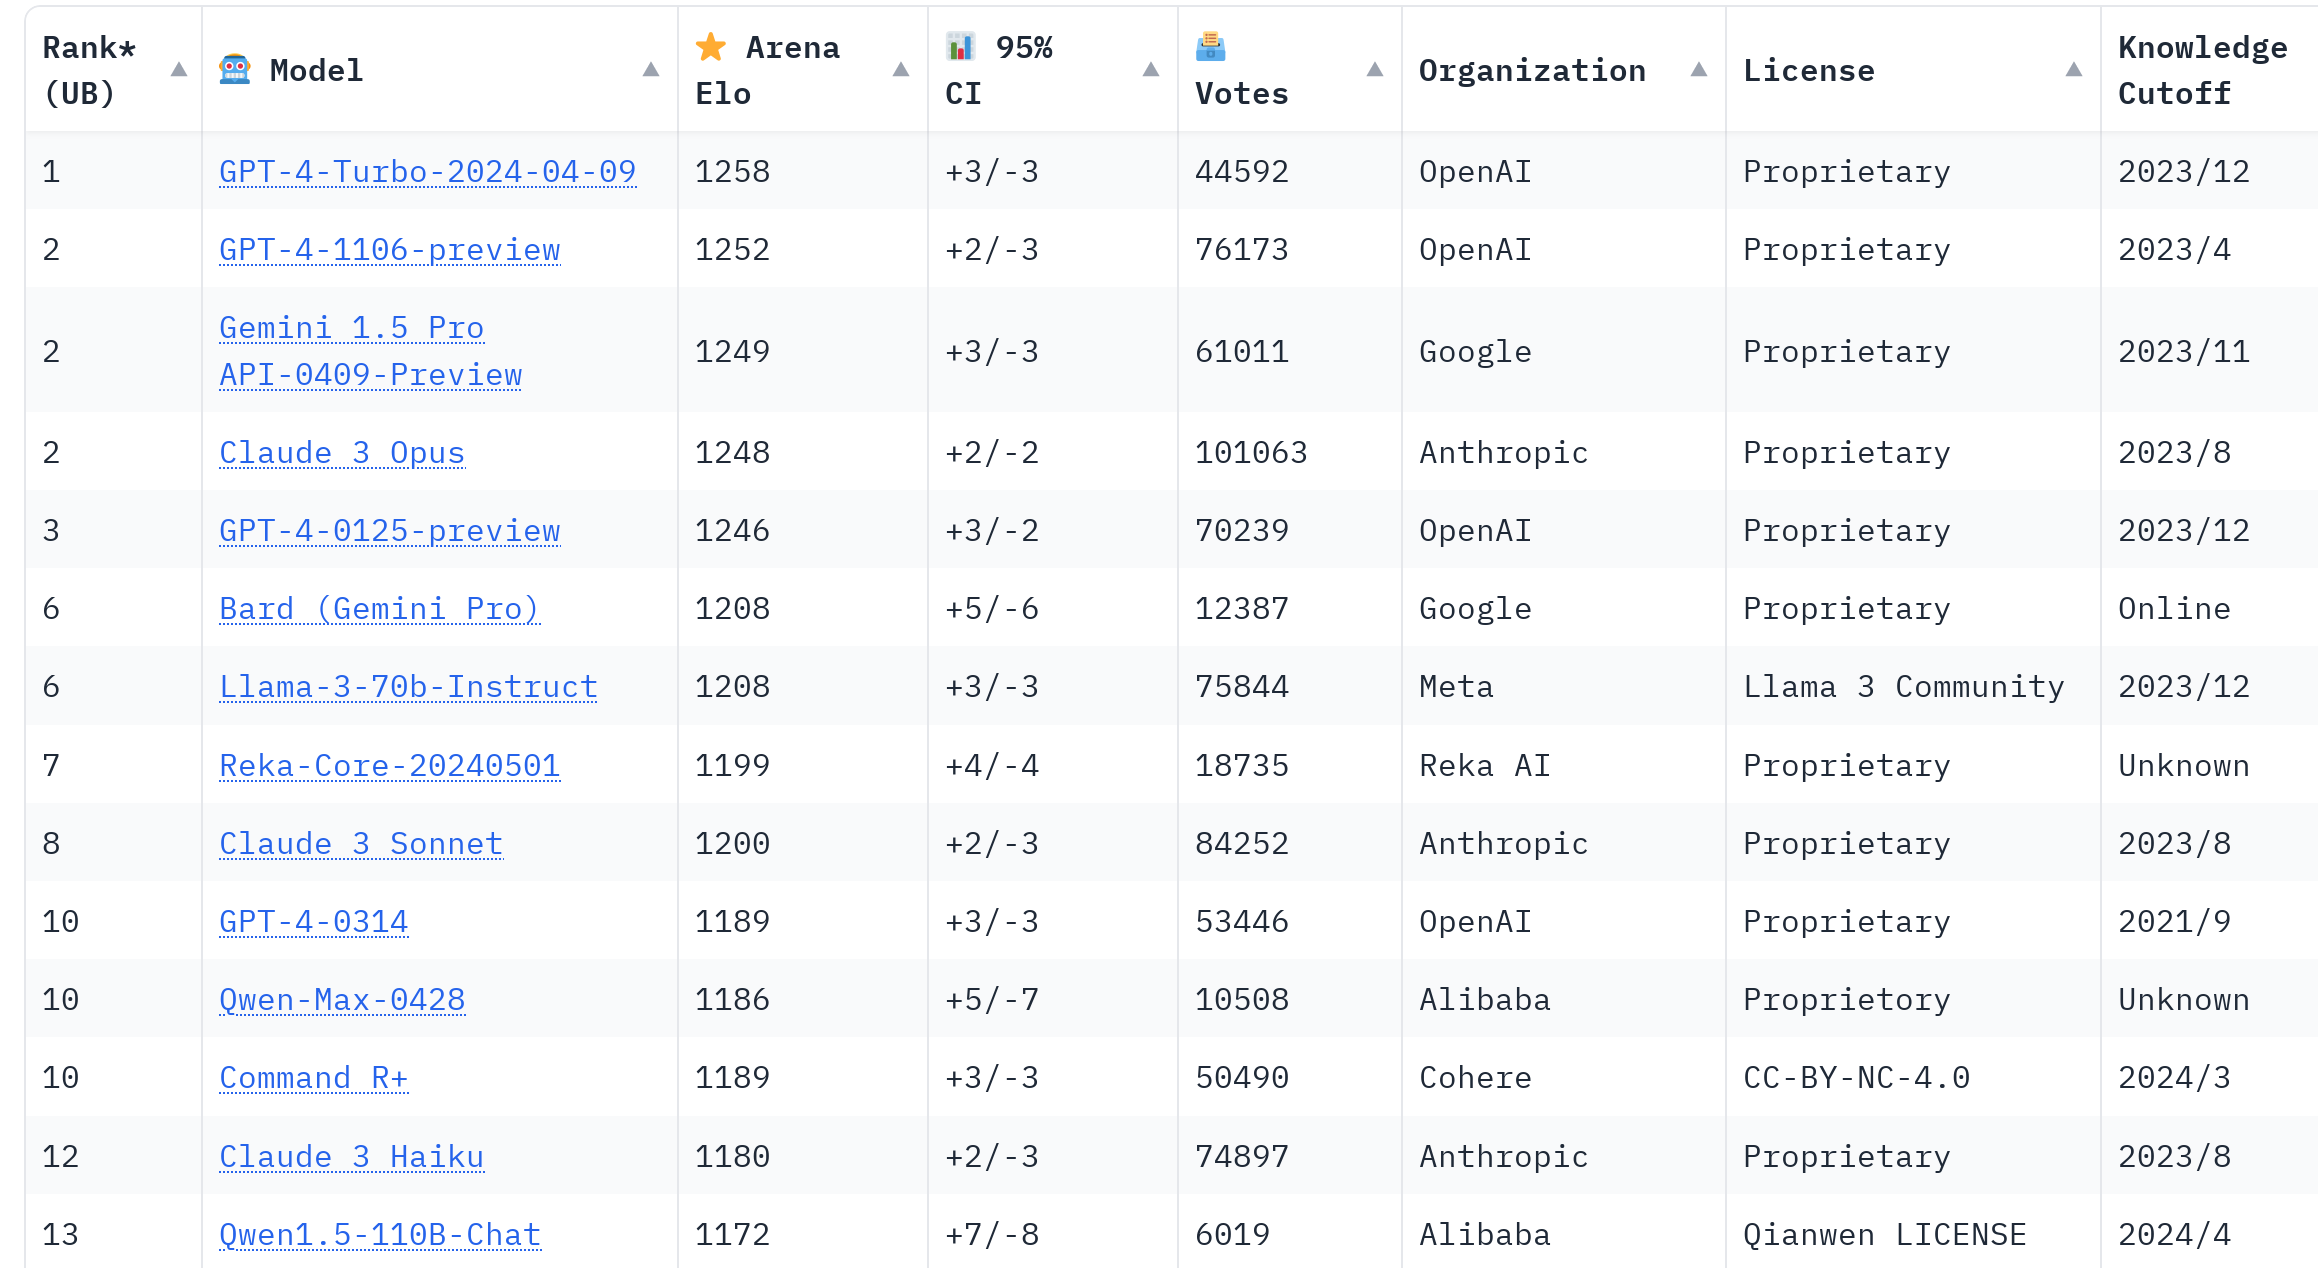
\includegraphics[width=7cm]{figs/leaderboard}

\url{https://lmarena.ai/?leaderboard}

\end{frame}

%% -----------------------------------------
\begin{frame}[fragile]
\frametitle{Motores de inferencia}

llama.cpp

\begin{flushright}
\url{https://github.com/ggerganov/llama.cpp}
\end{flushright}

Ollama

\begin{flushright}
\url{https://ollama.com/}
\end{flushright}

vLLM

\begin{flushright}
\url{https://github.com/vllm-project/vllm}
\end{flushright}

\end{frame}

%% -----------------------------------------
\begin{frame}[fragile]
\frametitle{Interfaces de chat}

Oobabooga:
\begin{flushright}
\url{https://github.com/oobabooga/text-generation-webui}
\end{flushright}

openplayground:
\begin{flushright}
\url{https://github.com/nat/openplayground}
\end{flushright}

catAI
\begin{flushright}
\url{https://github.com/withcatai/catai}
\end{flushright}

\end{frame}

%%-----------------------------------------
\begin{frame}[fragile]
\frametitle{Colecciones de datos consentidos y abiertos}

Chatbot Arena Leaderboard \\
\url{https://chat.lmsys.org/}

LAION Open Empathic \\
\url{https://laion.ai/blog/open-empathic/}

Conjuntos de datos LAION \\
\url{https://laion.ai/projects/}
\end{frame}

%%-----------------------------------------
\begin{frame}[fragile]
\frametitle{Marcos de agentes}

Camel--AI Owl \\
{\small \url{https://github.com/camel-ai/owl} \\
\url{https://github.com/camel-ai}}

LangChain \\
{\small \url{https://langchain.com/}}

Smolagents \\
{\small \url{https://github.com/huggingface/smolagents}}
\end{frame}

% %%-----------------------------------------
% %%-----------------------------------------
% \section{Extending, combining}

% %%-----------------------------------------
% \begin{frame}[fragile]
% \frametitle{Integration: GIMP}

% \begin{center}
% 
\includegraphics[width=7cm]{figs/sd-gimp}
% \end{center}

% \begin{flushright}
% {\scriptsize
% \url{https://github.com/blueturtleai/gimp-stable-diffusion} \
% }
% \end{flushright}

% \end{frame}

% %%-----------------------------------------
% \begin{frame}[fragile]
% \frametitle{Integration: Blender}

% \begin{center}
% 
\includegraphics[width=7cm]{figs/sd-blender}
% \end{center}

% \begin{flushright}
% {\scriptsize
% \url{https://blendermarket.com/products/ai-render} \
% }
% \end{flushright}

% \end{frame}

% %%-----------------------------------------
% \begin{frame}[fragile]
% \frametitle{In-painting}

% \begin{center}
% 
\includegraphics[width=9.5cm]{figs/sd-inpainting}
% \end{center}

% \begin{flushright}
% {\scriptsize
% \url{https://huggingface.co/spaces/multimodalart/stable-diffusion-inpainting} \
% }
% \end{flushright}

% \end{frame}

% %%-----------------------------------------
% \begin{frame}[fragile]
% \frametitle{Out-painting}

% \begin{center}
% 
\includegraphics[width=9.5cm]{figs/sd-infinity}
% \end{center}

% \begin{flushright}
% {\scriptsize
% \url{https://github.com/lkwq007/stablediffusion-infinity} \
% }
% \end{flushright}

% \end{frame}

% %% -----------------------------------------
% \begin{frame}[fragile]
% \frametitle{Image to image}

% Image + prompt produces an image \
% Even just with CPU! \

% \begin{flushright}
% {\scriptsize
% \url{https://huggingface.co/spaces/fffiloni/stable-diffusion-img2img} \
% }
% \end{flushright}

% \end{frame}

% %%-----------------------------------------
% \begin{frame}[fragile]

% \begin{center}
% 
\includegraphics[width=9.5cm]{figs/sd-mountains}
% \end{center}

% \begin{flushright}
% {\scriptsize
% \url{https://huggingface.co/spaces/huggingface-projects/diffuse-the-rest} \
% }
% \end{flushright}

% \end{frame}

% %% -----------------------------------------
% \begin{frame}[fragile]
% \frametitle{Multilingual AI Assistant}

% Whisper for Speech-to-text \
% Bloom for Text-generation, \
% CoquiTTS for Text-To-Speech \

% \begin{flushright}
% {\scriptsize
% \url{https://huggingface.co/spaces/ysharma/Talk_to_Multilingual_AI_WhisperBloomCoqui} \
% }
% \end{flushright}

% \end{frame}

% %% -----------------------------------------
% \begin{frame}[fragile]
% \frametitle{Whisper to Stable Diffusion}

% \begin{flushright}
% {\scriptsize
% \url{https://huggingface.co/spaces/fffiloni/whisper-to-stable-diffusion} \
% }
% \end{flushright}

% \end{frame}

% %%-----------------------------------------
% \begin{frame}[fragile]
% \frametitle{Whisper for YouTube captions}

% 
\includegraphics[width=8.5cm]{figs/whisper-youtube}

% \begin{flushright}
% {\scriptsize
% \url{https://github.com/openai/whisper/discussions/239}
% }
% \end{flushright}

% \end{frame}

% %%-----------------------------------------
% \begin{frame}[fragile]

% \begin{center}
% {\Large Y mucho, mucho más}
% \end{center}

% \end{frame}

% %%-----------------------------------------
% \begin{frame}[fragile]
% \frametitle{Un cuento (1): LLaMa}

% 25 de febrero de 2023 / Licencia: uso en investigación

% 
\includegraphics[height=3.5cm]{figs/llama}

% \begin{flushright}
% {\scriptsize
% \url{https://ai.facebook.com/blog/large-language-model-llama-meta-ai/}
% }
% \end{flushright}

% \end{frame}

% %%-----------------------------------------
% \begin{frame}[fragile]
% \frametitle{Un cuento (2): Dalai}

% 12 de marzo de 2023

% \begin{columns}[T]
% \begin{column}{.58\textwidth}
% 
\includegraphics[width=7.5cm]{figs/dalai}
% \end{column}%
% \hfill%
% \begin{column}{.38\textwidth}
% \vspace{1.5cm}

% Módulo de JavaScript que proporciona una interfaz web para LLaMA (y más tarde Alpaca)

% Licencia: ??

% {\scriptsize
% \url{https://github.com/antimatter15/alpaca.cpp}
% }
% \end{column}%
% \end{columns}

% \end{frame}

% %%-----------------------------------------
% \begin{frame}[fragile]
% \frametitle{Un cuento (3): Alpaca}

% 13 de marzo de 2023

% \begin{quote}
% \footnotesize ``Un grupo [...] en la Universidad de Stanford ajustó LLaMA para desarrollar Alpaca, un modelo de siete mil millones de parámetros de código abierto que costó menos de 600 dólares construir. [...] algunos [desarrolladores] lograron ejecutarlo en computadoras Raspberry Pi e incluso en un smartphone Pixel 6.''
% \end{quote}

% Licencia: uso en investigación (conjunto de datos: CC-BY-NC)

% \begin{flushright}
% {\scriptsize
% \url{https://github.com/tatsu-lab/stanford_alpaca} \
% \url{https://crfm.stanford.edu/2023/03/13/alpaca.html} \
% \url{https://theregister.com/2023/03/21/stanford_ai_alpaca_taken_offline/} \
% }
% \end{flushright}
% \end{frame}

% %%-----------------------------------------
% \begin{frame}[fragile]
% \frametitle{Un cuento (4): Serge}

% \begin{columns}[T]
% \begin{column}{.58\textwidth}
% 
\includegraphics[width=7.5cm]{figs/serge}
% \end{column}%
% \hfill%
% \begin{column}{.38\textwidth}
% \vspace{1.5cm}

% Contenedores Docker para desplegar un chat con modelos LLaMa (Alpaca)

% {\scriptsize
% \url{https://github.com/nsarrazin/serge}
% }
% \end{column}%
% \end{columns}

% \end{frame}

% %%-----------------------------------------
% \begin{frame}[fragile]
% \frametitle{Un cuento (5): Alpaca Electron}

% \begin{columns}[T]
% \begin{column}{.58\textwidth}
% 
\includegraphics[width=7.5cm]{figs/alpaca-electron}
% \end{column}%
% \hfill%
% \begin{column}{.38\textwidth}
% \vspace{1.5cm}

% Aplicación Electron para desplegar un chat con modelos LLaMa (Alpaca)

% {\scriptsize
% \url{https://github.com/ItsPi3141/alpaca-electron}
% }
% \end{column}%
% \end{columns}

% \end{frame}

% %%-----------------------------------------
% \begin{frame}[fragile]
% \frametitle{Un cuento (6): OobaBooga}

% \begin{columns}[T]
% \begin{column}{.58\textwidth}
% 
\includegraphics[width=7.5cm]{figs/oobabooga}
% \end{column}%
% \hfill%
% \begin{column}{.38\textwidth}
% \vspace{1.5cm}

% OobaBooga proporciona una interfaz web fácil para muchos modelos.

% {\scriptsize
% \url{https://github.com/ItsPi3141/alpaca-electron}
% }
% \end{column}%
% \end{columns}

% \end{frame}

%%-----------------------------------------
%%-----------------------------------------
\section{Infraestructura para jugar, para compartir}

%%-----------------------------------------
\begin{frame}[fragile]
\frametitle{Hugging Face}

\begin{columns}[T]
\begin{column}{.58\textwidth}
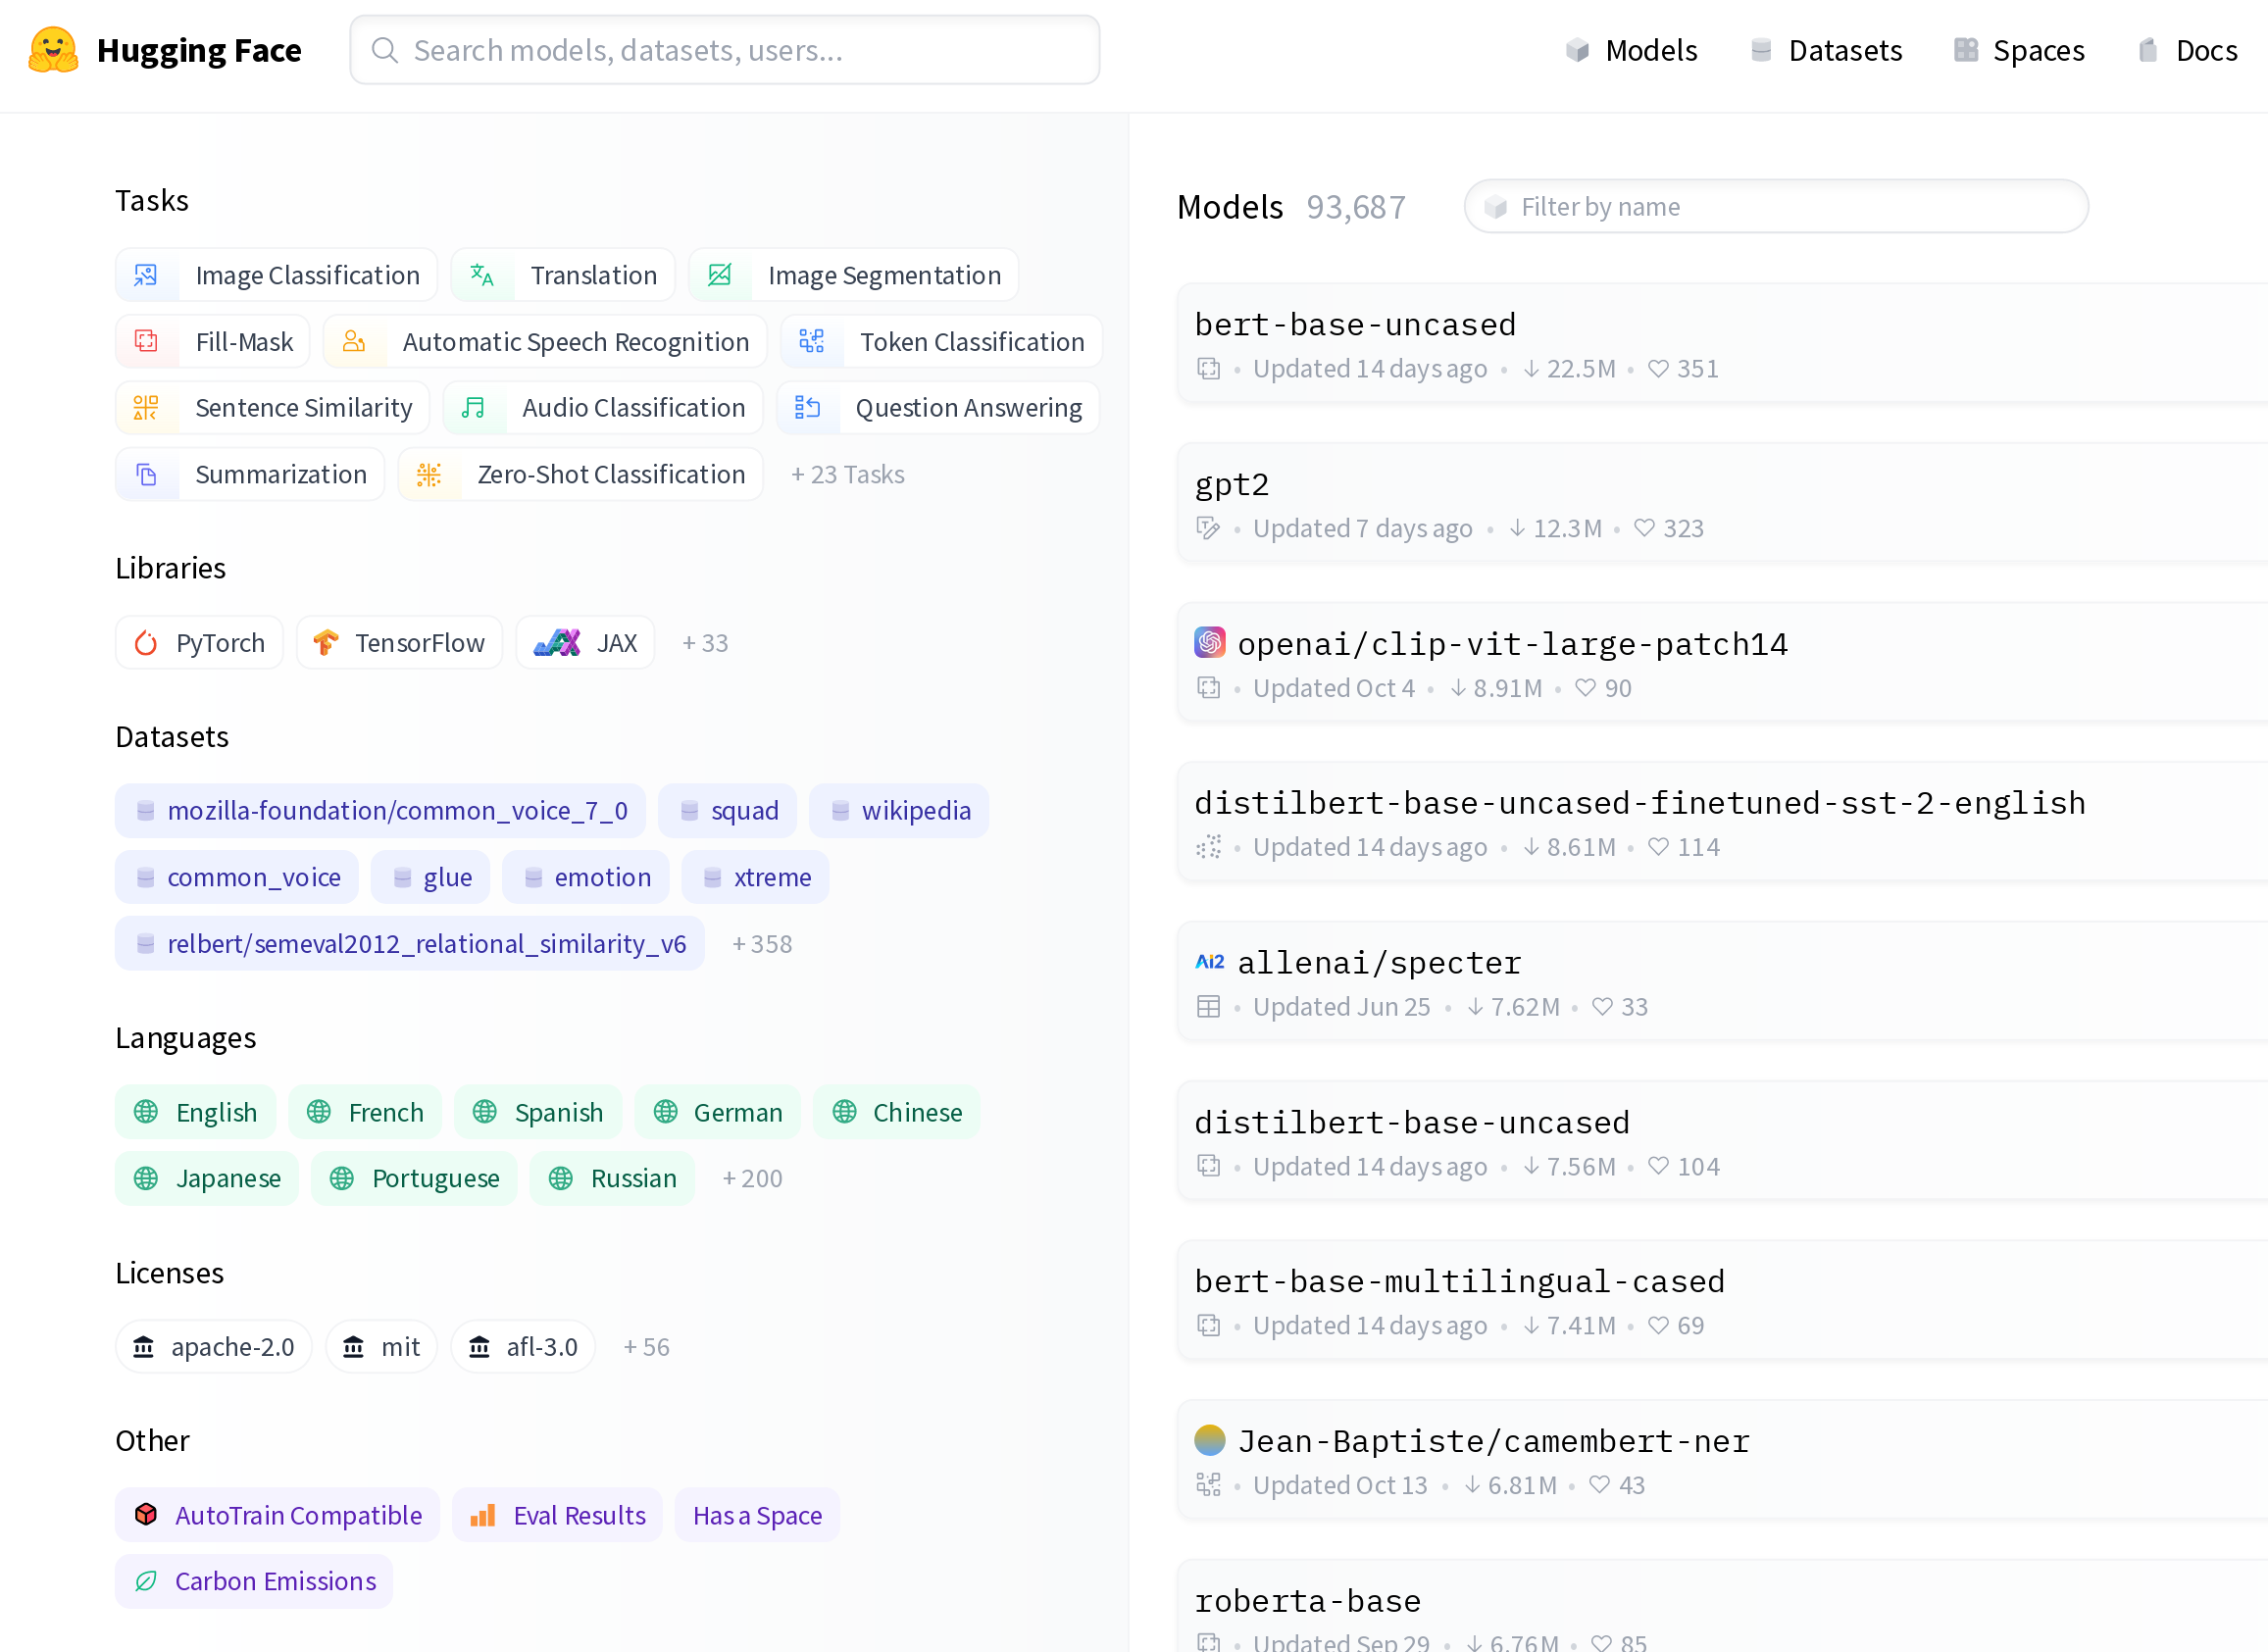
\includegraphics[width=7.5cm]{figs/hugging-face}
\end{column}%
\hfill%
\begin{column}{.38\textwidth}
``GitHub para ML''

    \vspace{2cm}
    
    {\scriptsize
      \url{https://huggingface.co} \\
    }
\end{column}%

\end{columns}

\end{frame}

%%-----------------------------------------
\begin{frame}[fragile]
\frametitle{Gradio}

\begin{center}
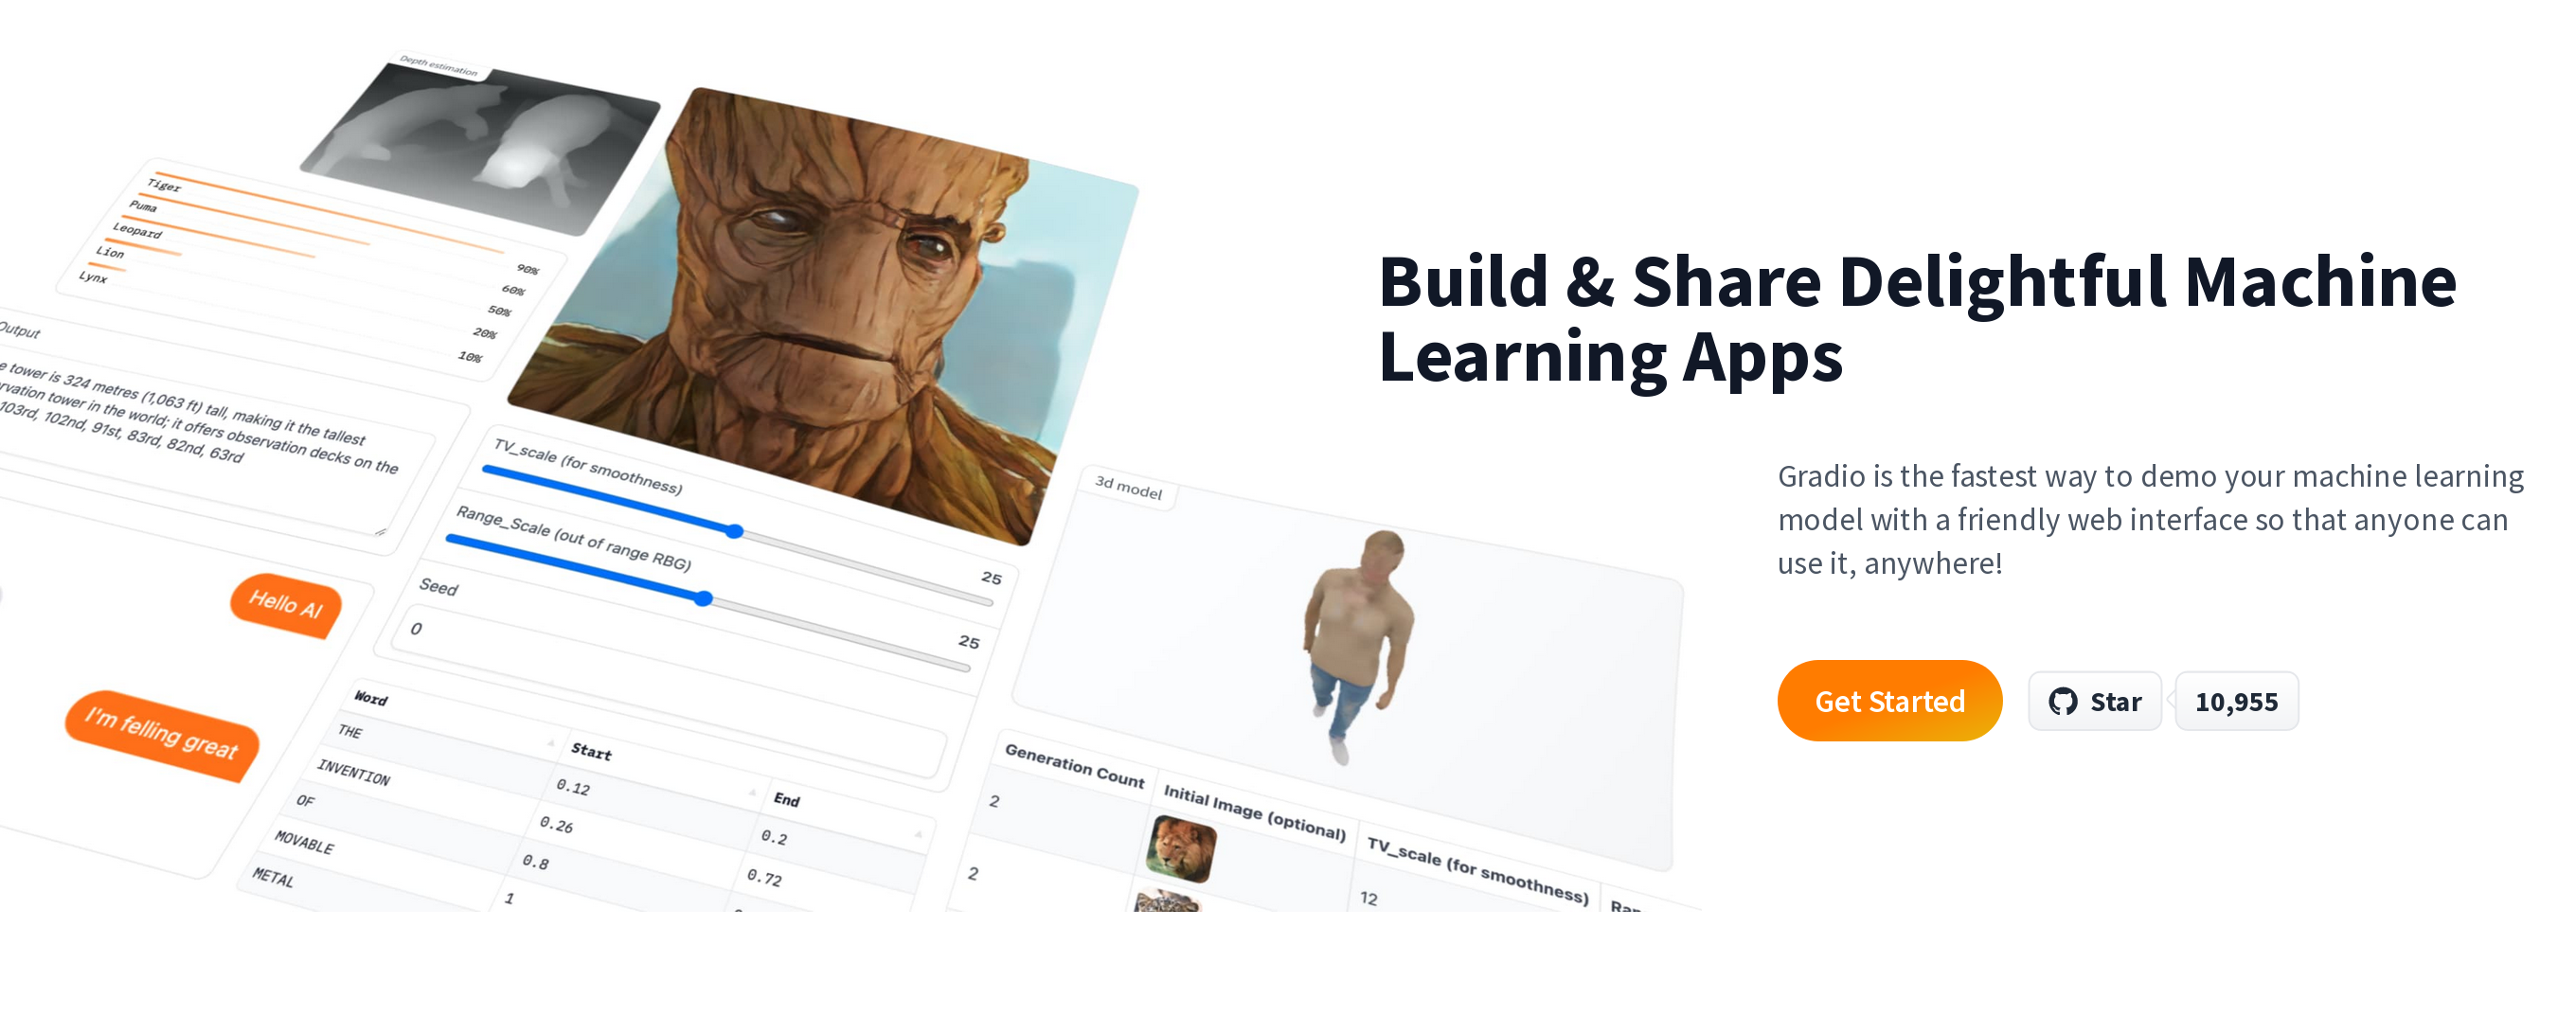
\includegraphics[width=12cm]{figs/gradio}
\end{center}

\begin{flushright}
{\small
\url{https://gradio.app/} \\
Licencia: Apache 2.0 \\
}
\end{flushright}
\end{frame}

%%-----------------------------------------
\begin{frame}[fragile]
\frametitle{Diffusers}

\begin{center}

\includegraphics[width=8cm]{figs/diffusers}
\end{center}

Modelos de difusión preentrenados (visión, audio, etc.) \\
Caja de herramientas modular para inferencia y entrenamiento de modelos de difusión \\

\begin{flushright}
{\small
\url{https://github.com/huggingface/diffusers} \\
Licencia: Apache 2.0 \\
}
\end{flushright}
\end{frame}

%%-----------------------------------------
\begin{frame}[fragile]
\frametitle{Marcos de modelos, etc.}

\begin{columns}[T]
\begin{column}{.28\textwidth}

\begin{flushright}
PyTorch
\end{flushright}

\begin{flushright}
TensorFlow
\end{flushright}

\begin{flushright}
Keras
\end{flushright}

\begin{flushright}
Cuda
\end{flushright}
\end{column}%
\hfill%
\begin{column}{.68\textwidth}
\begin{flushright}
{\small \url{https://pytorch.org/}}
\end{flushright}

\begin{flushright}
{\small \url{https://tensorflow.org/}}
\end{flushright}

\begin{flushright}
{\small \url{https://keras.io/}}
\end{flushright}

\begin{flushright}
{\small  \url{https://developer.nvidia.com/cuda-toolkit}}

\end{flushright}
\end{column}%
\end{columns}

\end{frame}

%%-----------------------------------------
\begin{frame}[fragile]
\frametitle{Collab}

\begin{center}
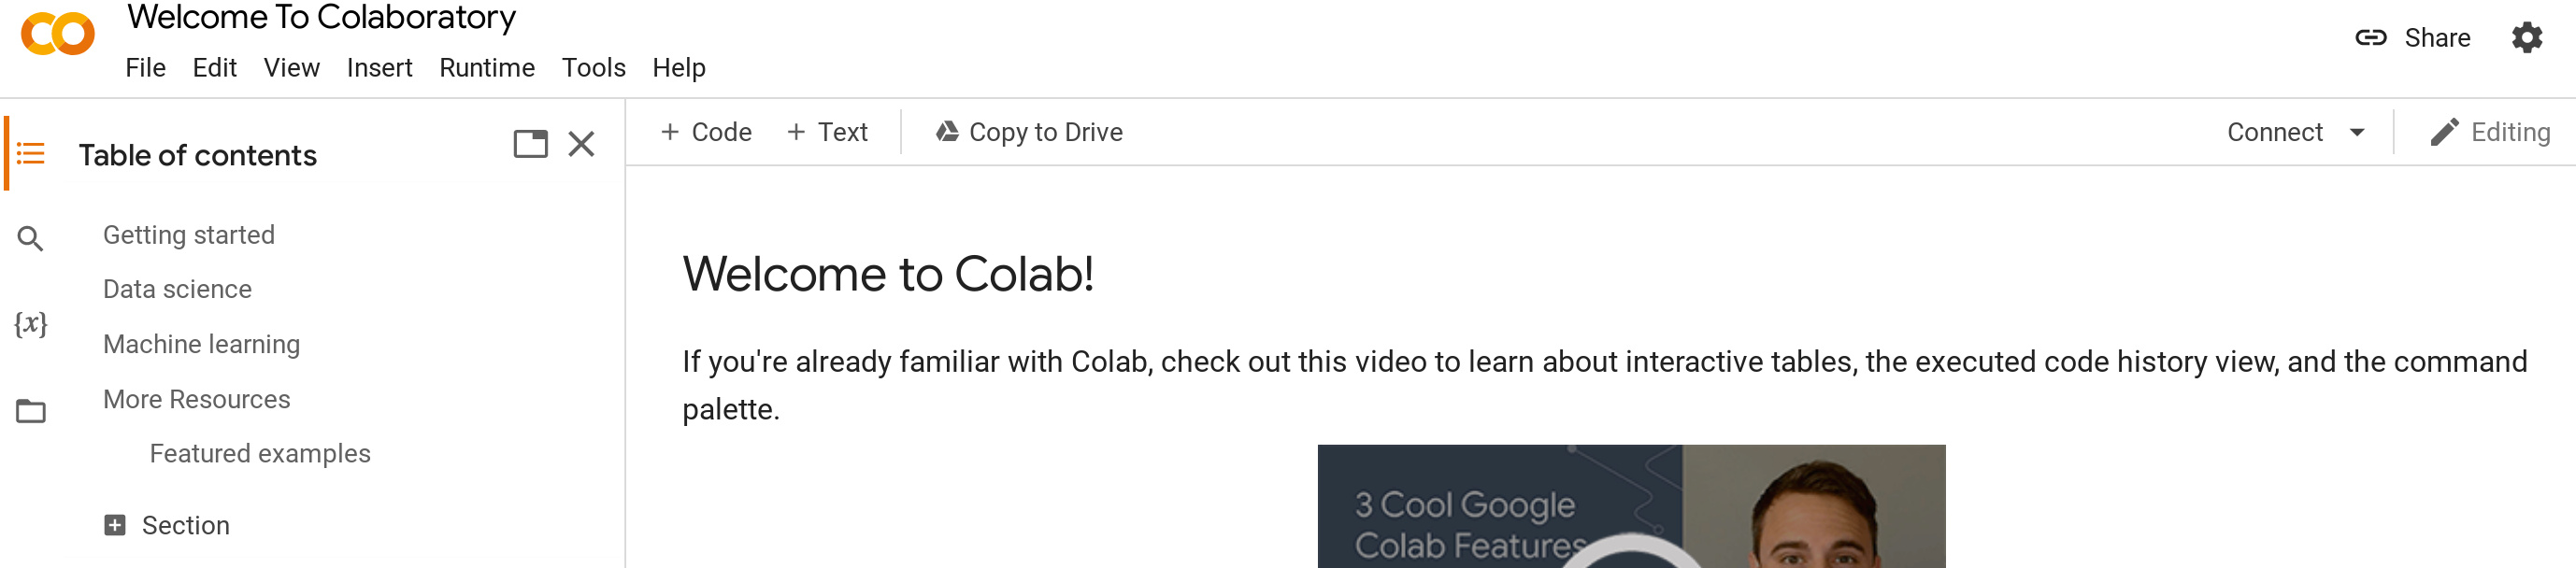
\includegraphics[width=12cm]{figs/collab}
\end{center}

Python en el navegador, cero configuración \\
Acceso a GPUs y fácil compartir \\

\begin{flushright}
{\small
\url{https://colab.research.google.com/}
}
\end{flushright}
\end{frame}

%%-----------------------------------------
\begin{frame}[fragile]
\frametitle{Jupyter}

\begin{center}

\includegraphics[width=10cm]{figs/jupyter}
\end{center}

Python en el navegador, fácil

\begin{flushright}
{\small
\url{https://jupyter.org/}
}
\end{flushright}
\end{frame}

%%-----------------------------------------
\begin{frame}[fragile]
\frametitle{Proveedores de API}

OpenRouter: \url{https://openrouter.ai/} \\
Groq: \url{https://groq.com/} \\
Together.ai: \url{https://together.ai} \\
SambaNova \url{https://sambanova.ai/} \\
...y muchos más \\
\end{frame}

%%-----------------------------------------
%%-----------------------------------------
\section{Muchos problemas planteados}

%%-----------------------------------------
\begin{frame}[fragile]
\frametitle{Propiedad intelectual (conjunto de entrenamiento)}

\begin{columns}[T]
\begin{column}{.58\textwidth}
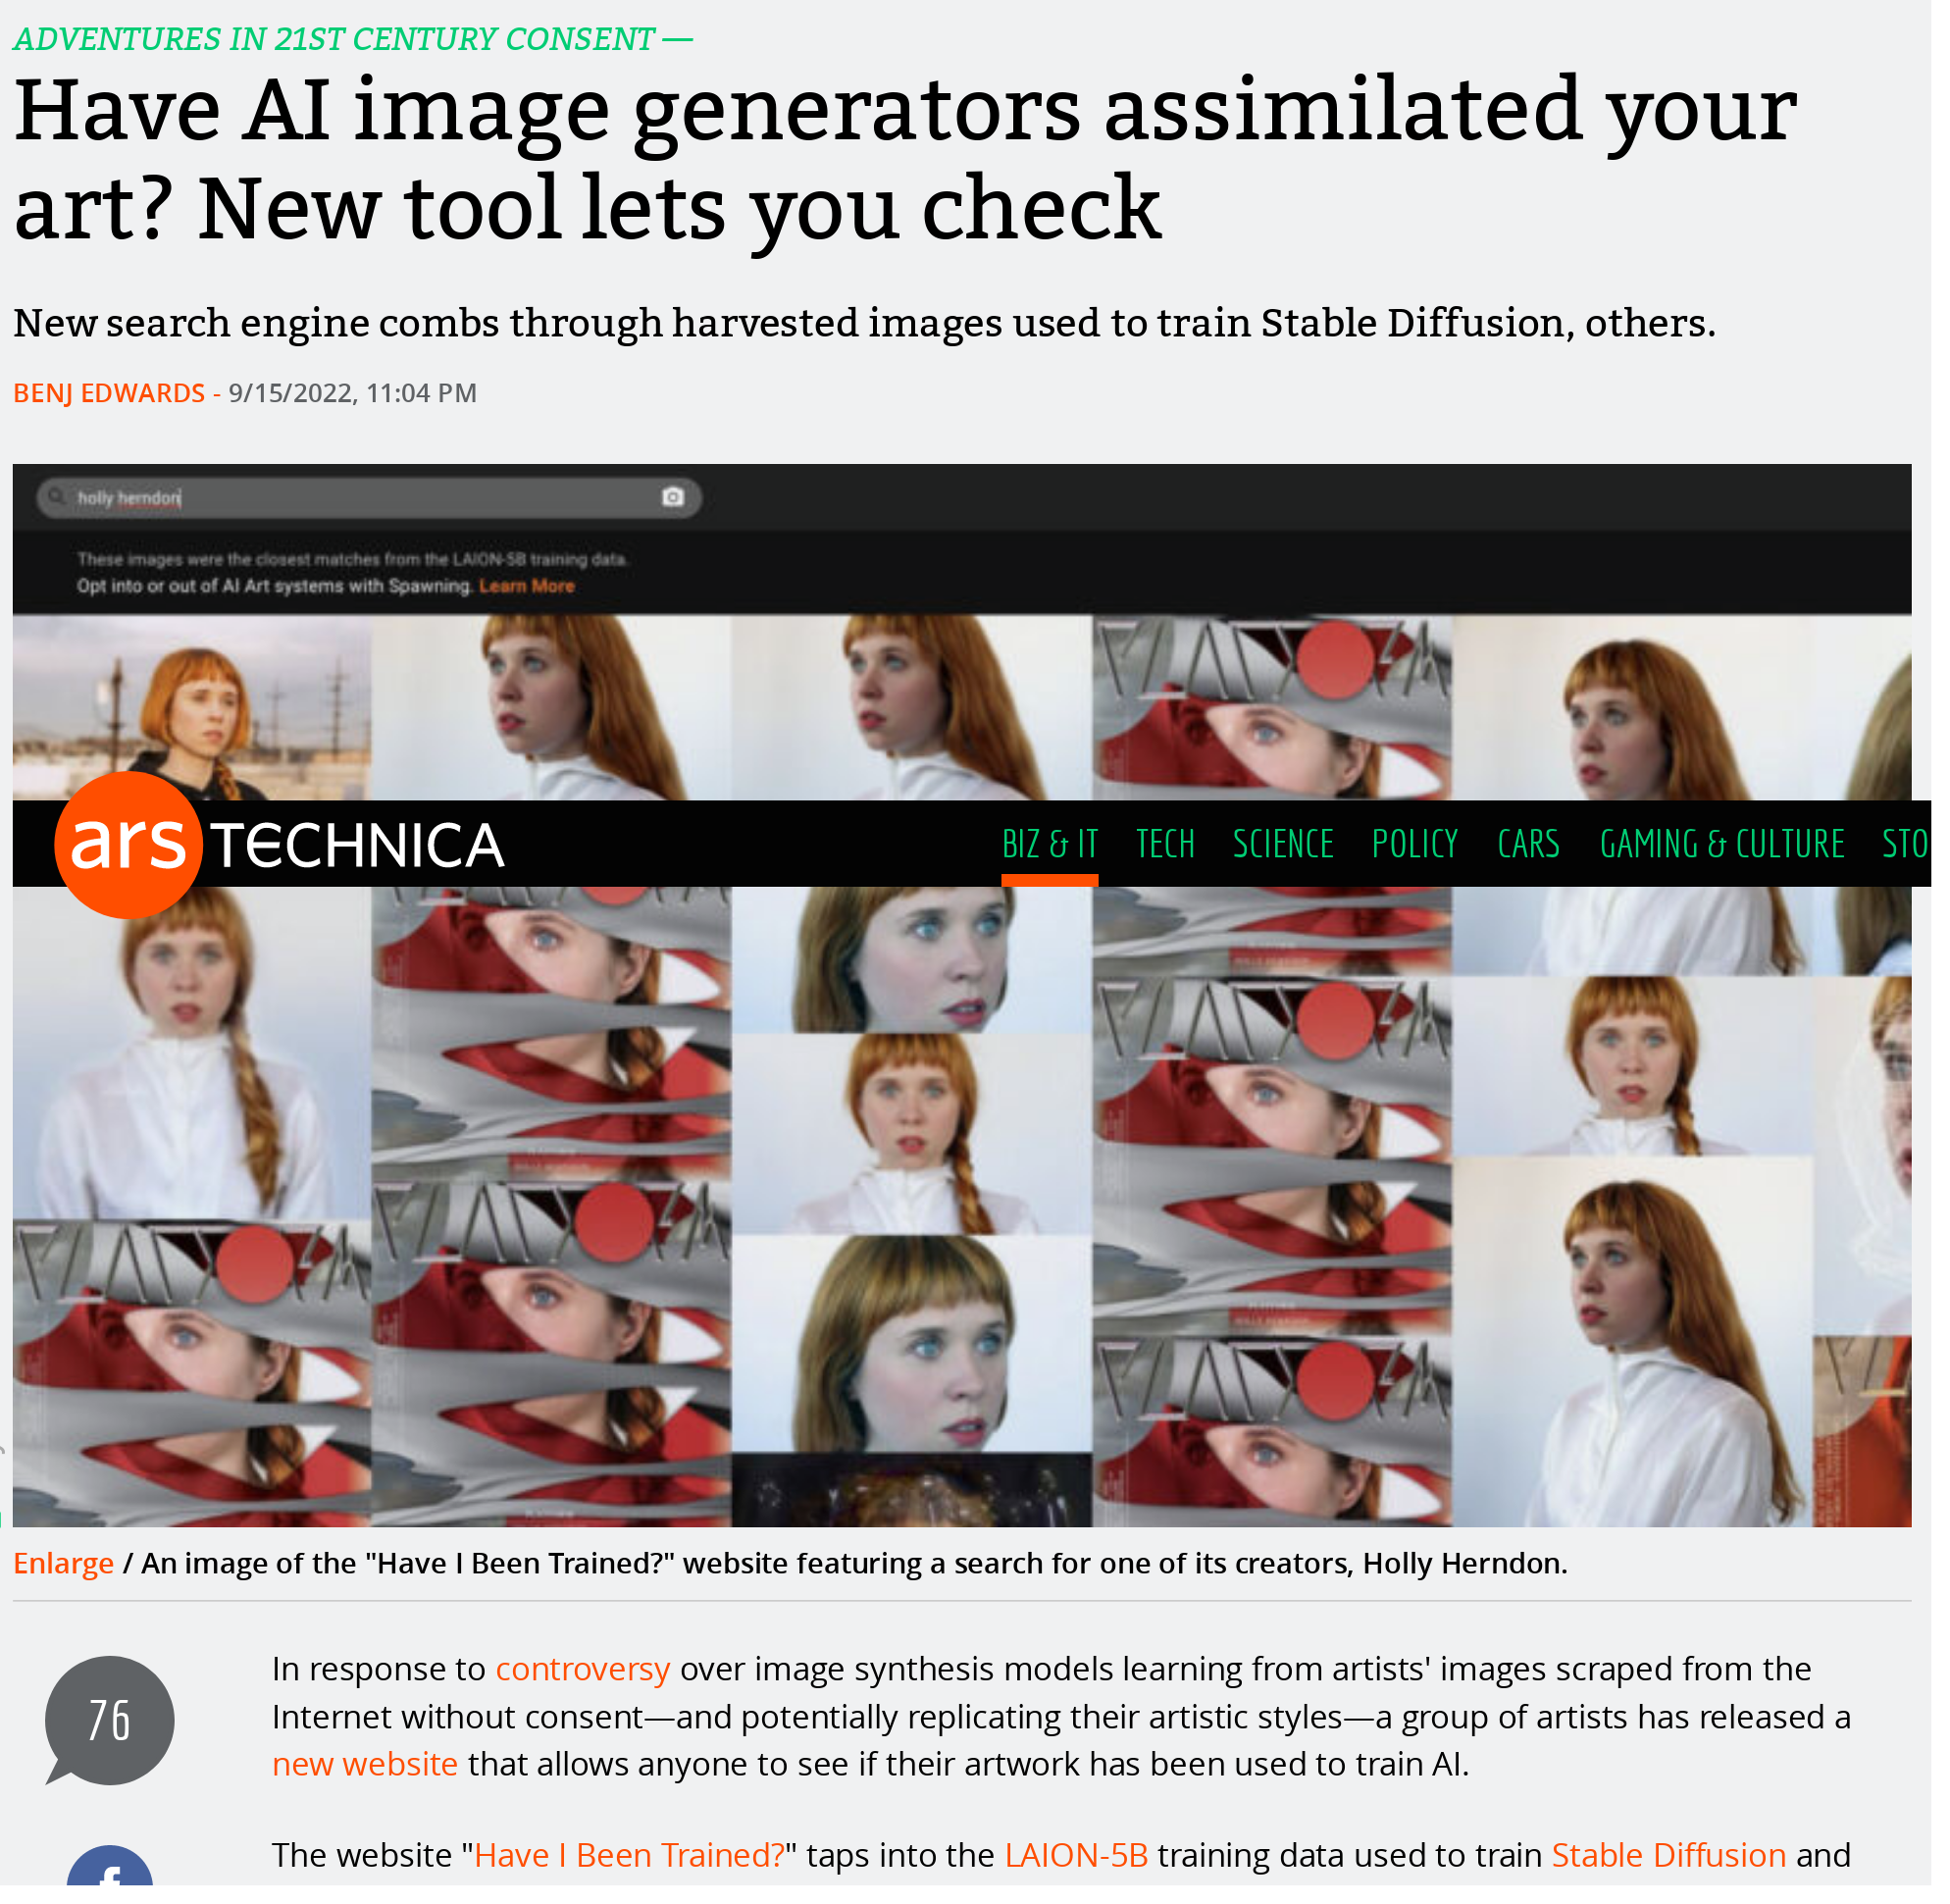
\includegraphics[width=7.5cm]{figs/used-art}
\end{column}%
\hfill%
\begin{column}{.38\textwidth}

    \vspace{0.5cm}
    
    {\scriptsize
      \url{https://haveibeentrained.com/} \\

      \vspace{1cm}
  
      \url{https://arstechnica.com/information-technology/2022/09/have-ai-image-generators-assimilated-your-art-new-tool-lets-you-check/} \\
    }
\end{column}%

\end{columns}

\end{frame}

%%-----------------------------------------
\begin{frame}[fragile]
\frametitle{Propiedad intelectual (resultados)}

    
\includegraphics[width=7.5cm]{figs/impact-ai-copyright}

    {\scriptsize
      \url{https://euipo.europa.eu/tunnel-web/secure/webdav/guest/document_library/observatory/documents/reports/2022_Impact_AI_on_the_Infringement_and_Enforcement_CR_Designs/2022_Impact_AI_on_the_Infringement_and_Enforcement_CR_Designs_FullR_en.pdf} \\
    }
    

\end{frame}

%%-----------------------------------------
\begin{frame}[fragile]
\frametitle{Propiedad intelectual}

\begin{itemize}
\item ¿Pueden los modelos entrenarse con cualquier cosa pública?

\item ¿Están los modelos sujetos a derechos de autor?

\item ¿Quién es el autor de la producción de un modelo?

\item ¿Puede alguien además del autor reclamar derechos sobre la producción de un modelo?
\end{itemize}

\end{frame}

%%-----------------------------------------
\begin{frame}[fragile]
\frametitle{Licencias}

\begin{columns}[T]
\begin{column}{.36\textwidth}
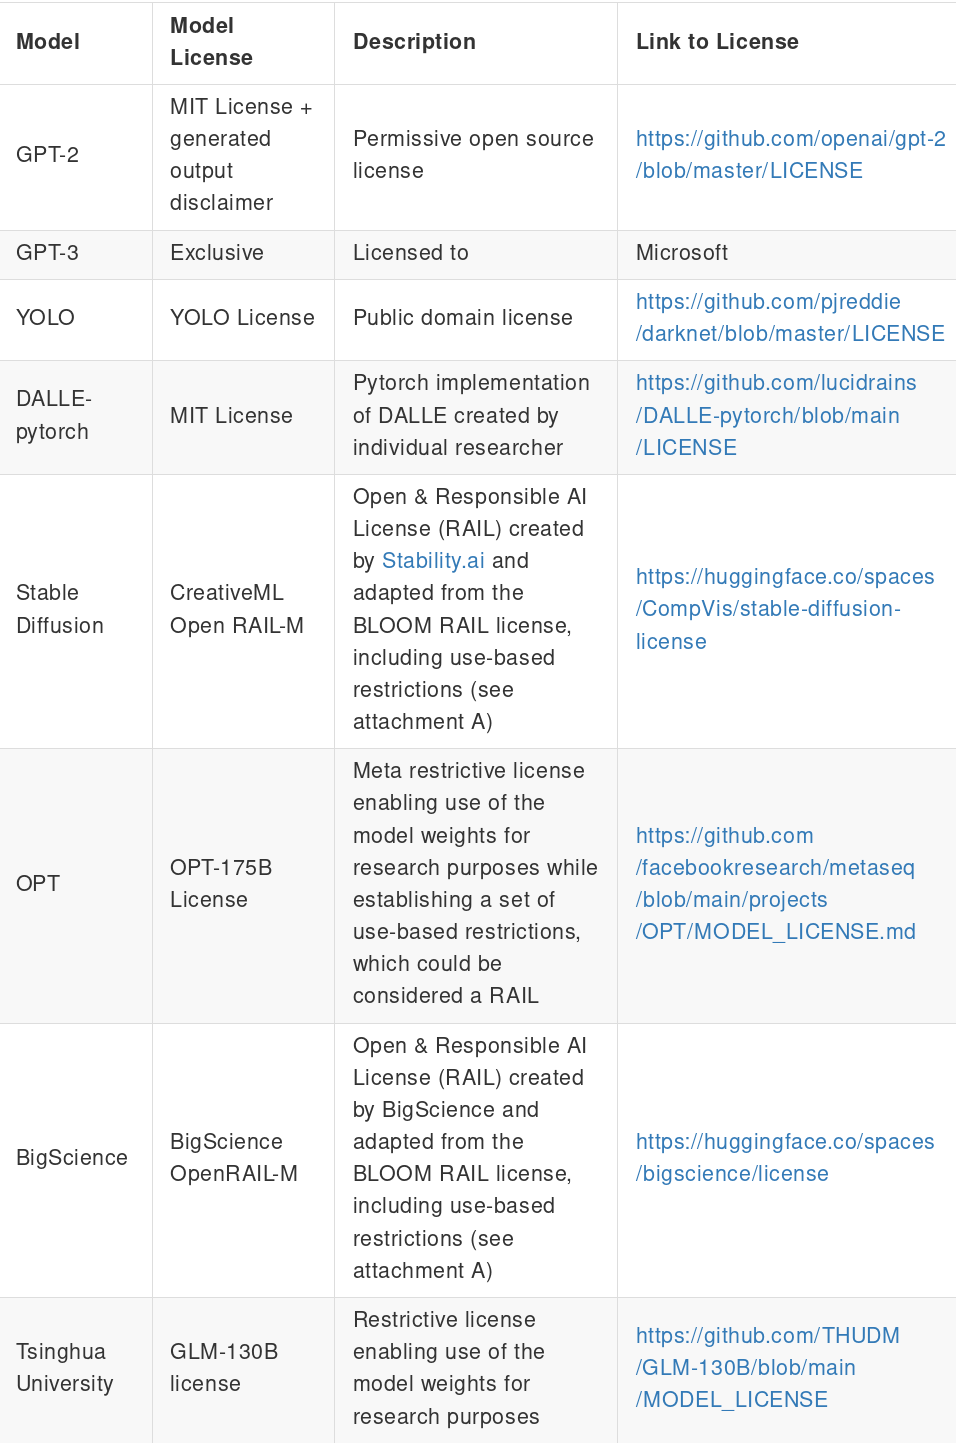
\includegraphics[width=4cm]{figs/licensing}
\end{column}%
\hfill%
\begin{column}{.62\textwidth}

    \vspace{0.5cm}
    
    {\scriptsize
      \url{https://hackmd.io/@jending12/HyvMU8sJo} \\

      \vspace{1.5cm}
      \url{https://thegradient.pub/machine-learning-ethics-and-open-source-licensing-2/}
    }
\end{column}%

\end{columns}

\end{frame}

%%-----------------------------------------
\begin{frame}[fragile]
\frametitle{Sesgo}

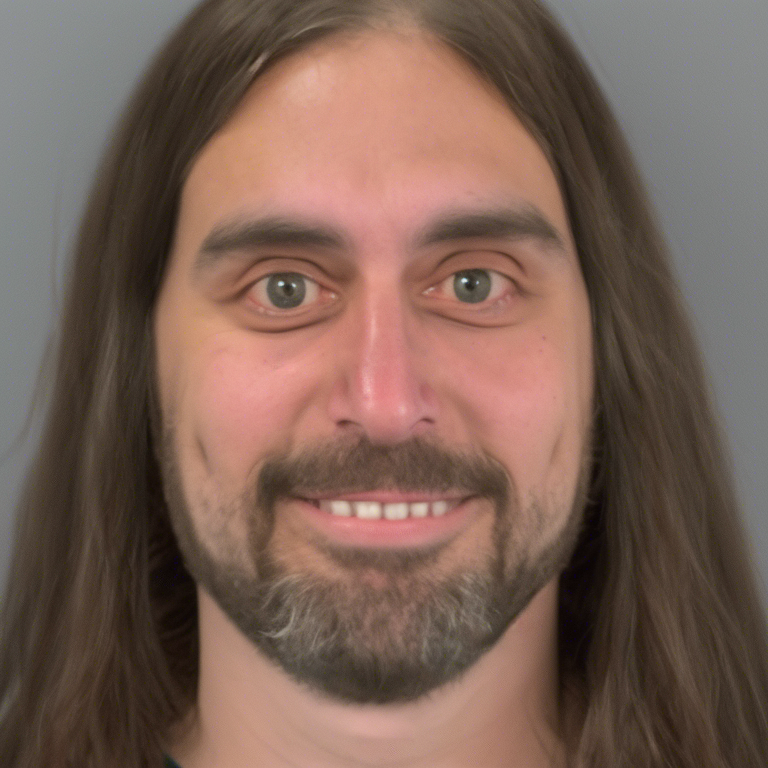
\includegraphics[width=2cm]{figs/17a}
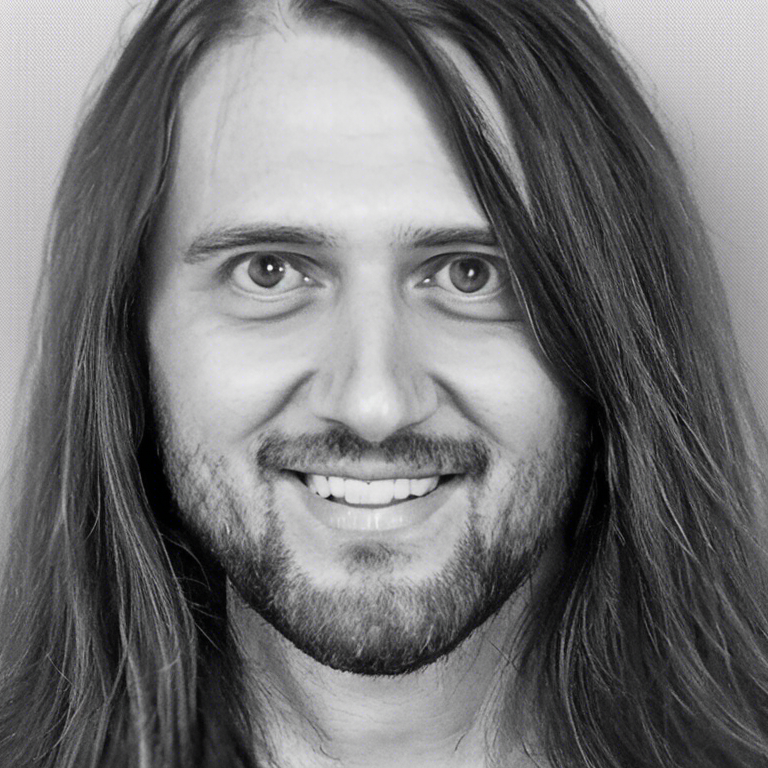
\includegraphics[width=2cm]{figs/17b}
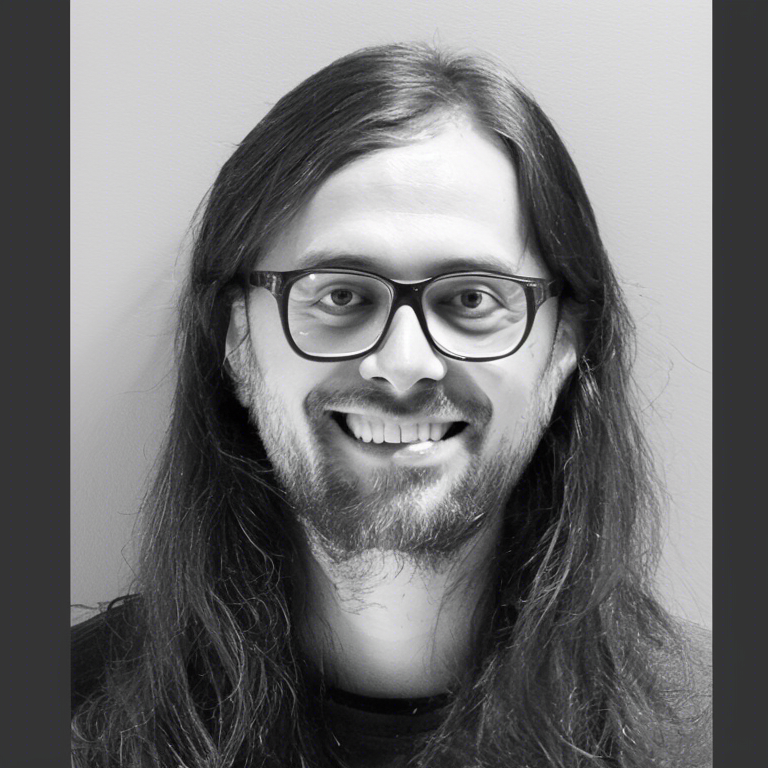
\includegraphics[width=2cm]{figs/17c}
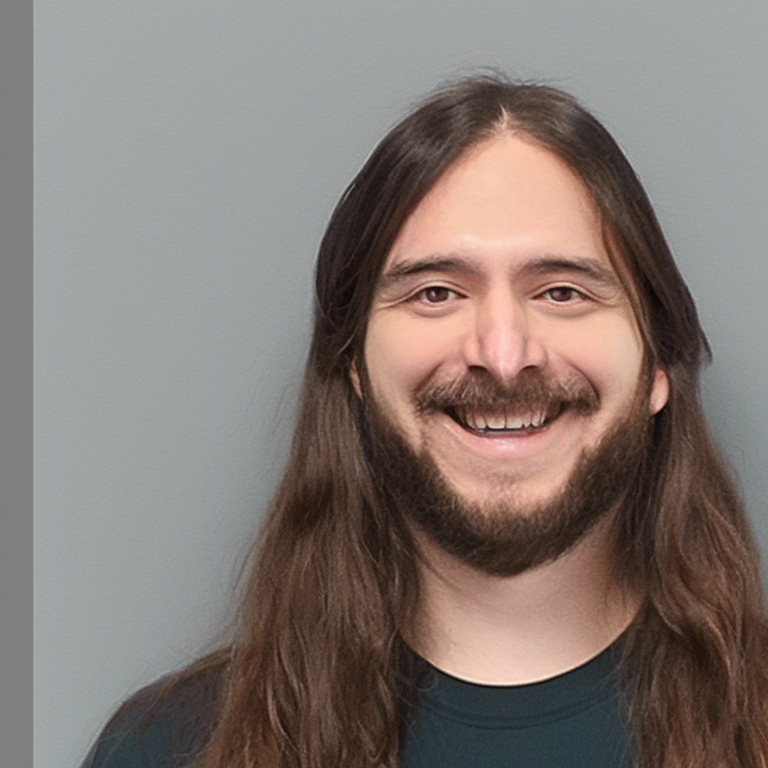
\includegraphics[width=2cm]{figs/17d}

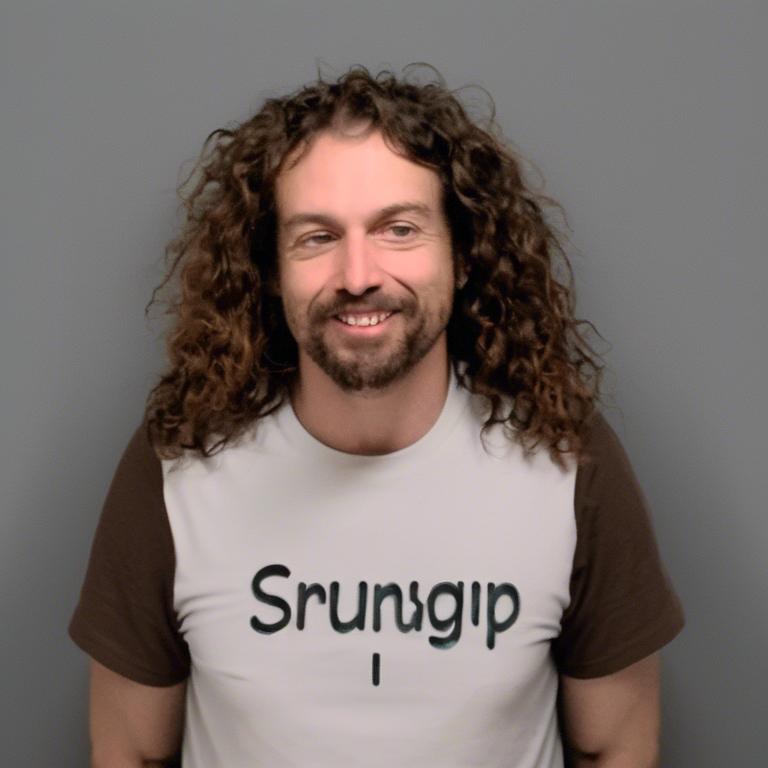
\includegraphics[width=2cm]{figs/18a}
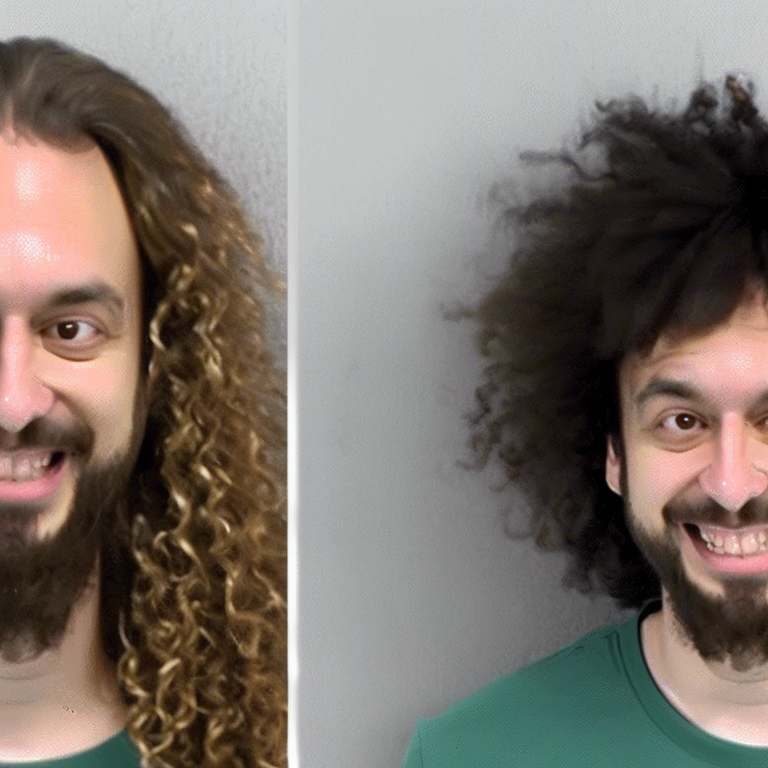
\includegraphics[width=2cm]{figs/18b}
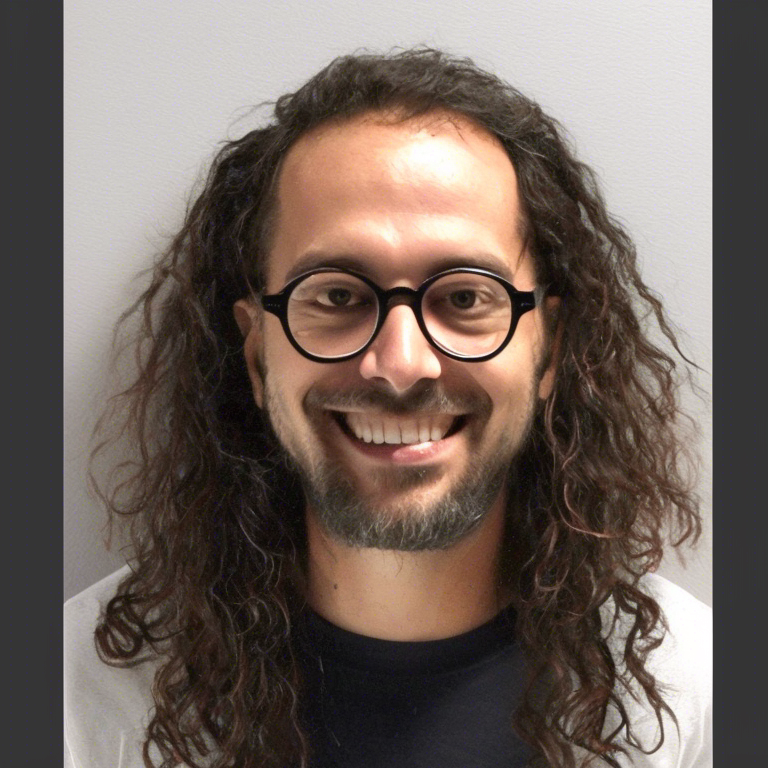
\includegraphics[width=2cm]{figs/18c}
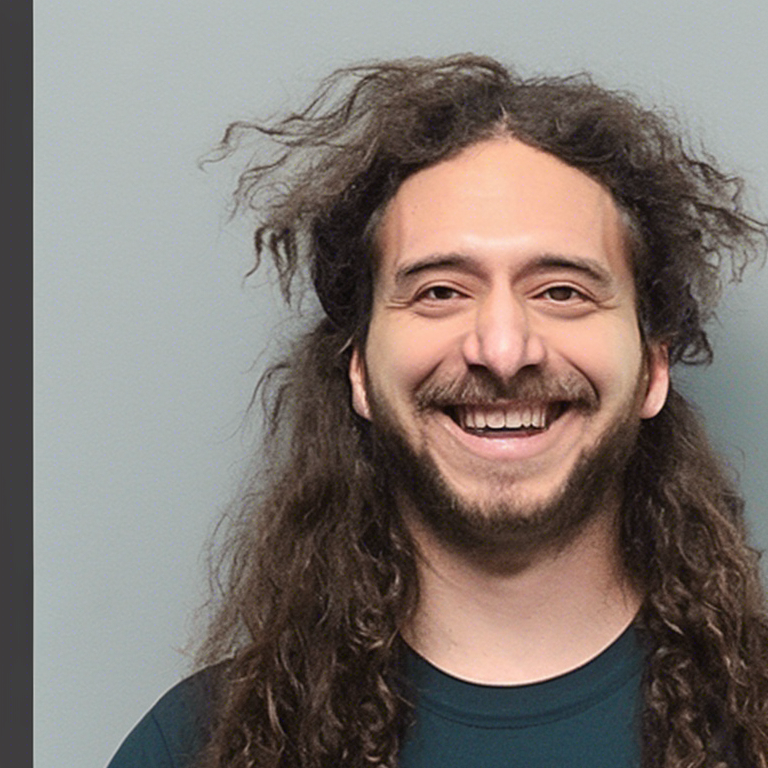
\includegraphics[width=2cm]{figs/18d}

{\small
  Fotografía de un ponente técnico, experto en aprendizaje automático, sonriendo, cabello largo, ojos grandes [camiseta, cabello rizado]
}

\end{frame}

%%-----------------------------------------
\begin{frame}[fragile]
\frametitle{Seguridad}


\includegraphics[width=9cm]{figs/ml-attacks}

{\scriptsize
\url{https://research.nccgroup.com/2022/07/06/whitepaper-practical-attacks-on-machine-learning-systems/} \\
\url{https://simonwillison.net/2022/Sep/12/prompt-injection/} \\
}

\end{frame}

%%-----------------------------------------
\begin{frame}[fragile]
\frametitle{Impacto en profesionales}

\begin{itemize}
\item ¿No más dibujar por encargo como profesión?
\item ¿Nuevas oportunidades para artistas?
\item ¿Acceso a modelos como necesidad fundamental?
\end{itemize}

¿Es esto diferente a la invención de la fotografía?
\end{frame}

%%-----------------------------------------
\begin{frame}[fragile]
\frametitle{Impacto en profesionales}

{\Large
¿Es esto diferente \\
de la invención de la fotografía? \\
}

\end{frame}

%%-----------------------------------------
\begin{frame}[fragile]
\frametitle{Ingenieros de prompts}

Una nueva profesión

\vspace{.5cm}

¿Artistas, ingenieros, artesanos?

\vspace{.5cm}

¿Permanecerá?

\end{frame}

%%-----------------------------------------
\begin{frame}[fragile]
\frametitle{¿Qué es cierto?}

\begin{center}
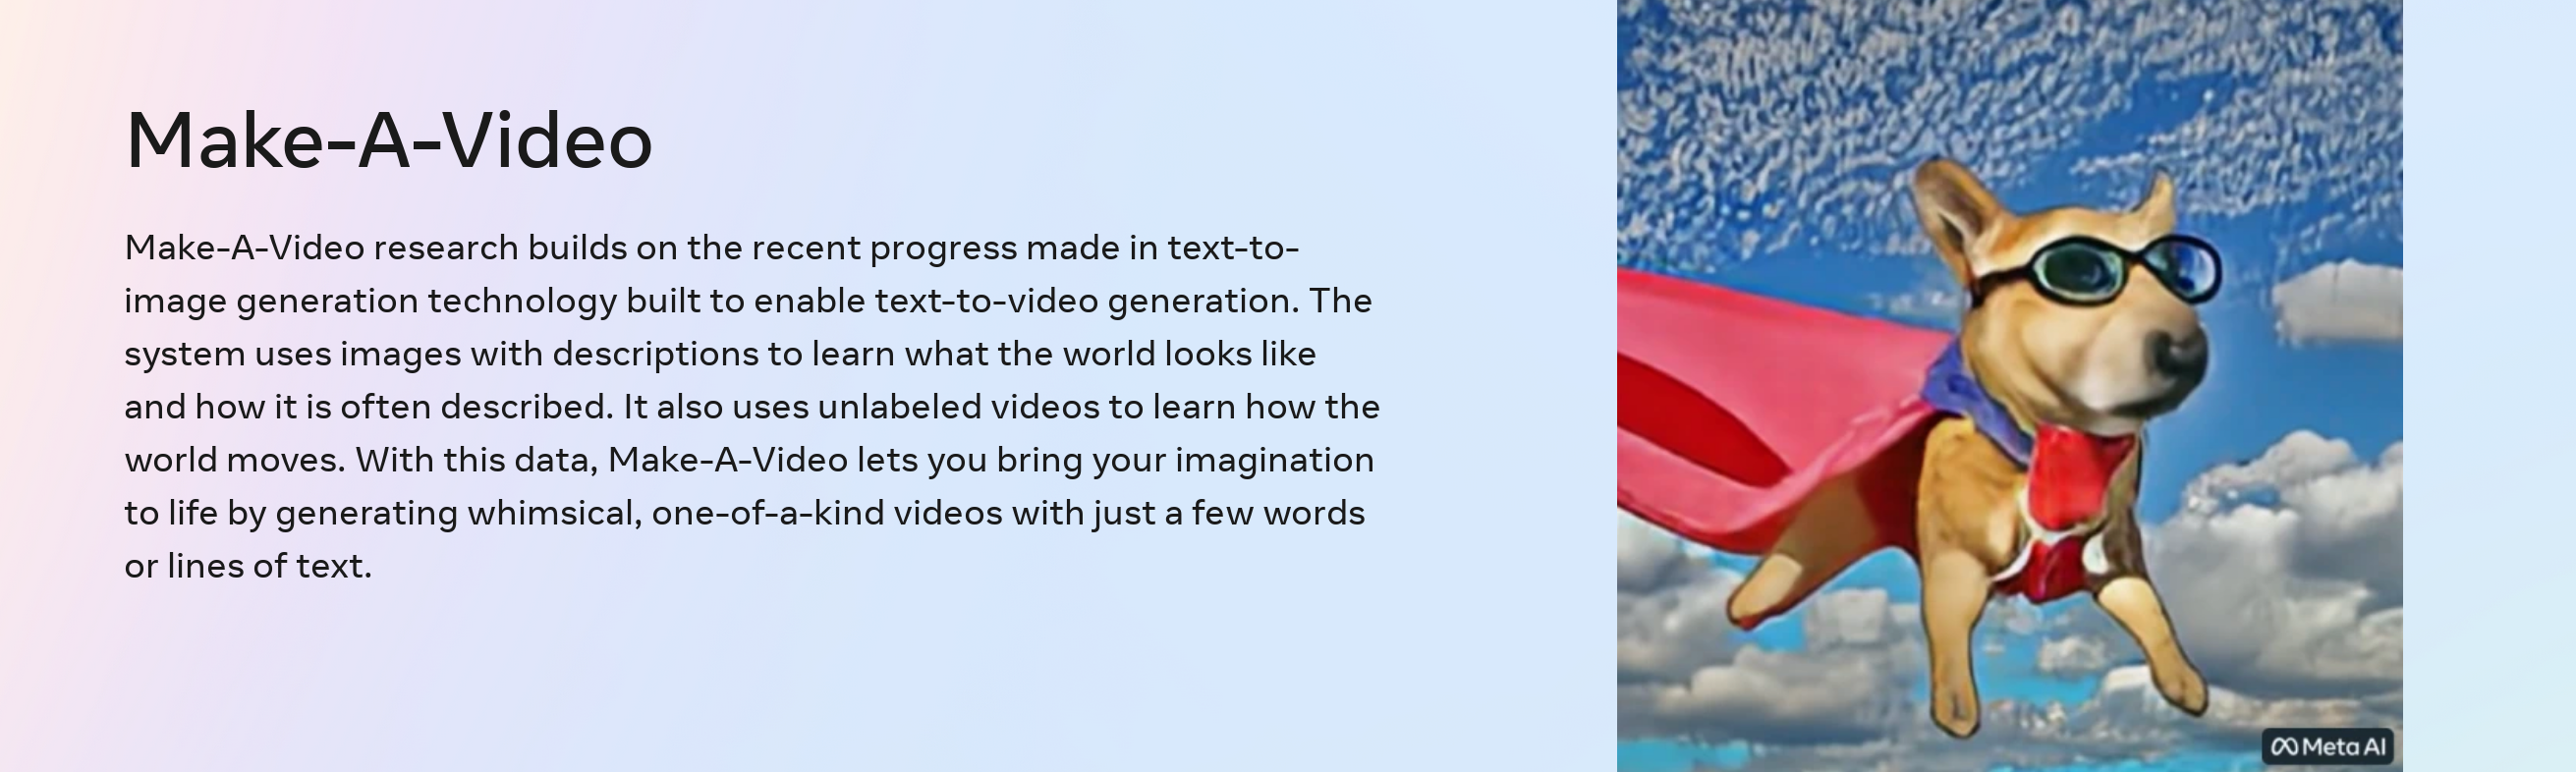
\includegraphics[width=9.5cm]{figs/makeavideo}

\end{center}

\begin{flushright}
{\scriptsize
\url{https://makeavideo.studio/}
}
\end{flushright}

\end{frame}

%%-----------------------------------------
%%-----------------------------------------
% \section{El futuro}

% %%-----------------------------------------
% \begin{frame}[fragile]
% \frametitle{Tareas}

% \begin{center}
% 
\includegraphics[width=7cm]{figs/kids-essays}
% \end{center}

% \end{frame}

% %%-----------------------------------------
% \begin{frame}[fragile]
% \frametitle{Programación}

% \begin{center}
% 
\includegraphics[width=10cm]{figs/llm-programming-better}
% \end{center}

% \begin{flushright}
% {\small
% \url{https://arxiv.org/abs/2207.14502}
% }
% \end{flushright}

% \end{frame}

% %%-----------------------------------------
% \begin{frame}[fragile]
% \frametitle{Programación}

% \begin{center}
% 
\includegraphics[width=10cm]{figs/self-programming}
% \end{center}

% \begin{flushright}
% {\scriptsize
% \url{https://keras.io/examples/generative/random_walks_with_stable_diffusion/}
% }
% \end{flushright}

% \end{frame}

%%-----------------------------------------
%%-----------------------------------------
\section{Resumiendo}

%% -----------------------------------------
\begin{frame}[fragile]

{\Large \bf
El futuro acaba de comenzar
}
\end{frame}

%%-----------------------------------------
%%-----------------------------------------
\section*{Referencias}

% -----------------------------------------
\begin{frame}[fragile]

{\huge Referencias, créditos, licencia}
\end{frame}

%% -----------------------------------------
\begin{frame}[fragile]
% \frametitle{Referencias}

{\small
\begin{itemize}
\item Transformers-Tutorials \\
{\scriptsize \url{https://github.com/NielsRogge/Transformers-Tutorials}}
\item Vision Transformers \\
{\scriptsize \url{https://cameronrwolfe.substack.com/p/vision-transformers}}
\item Un paseo por el espacio latente con Stable Diffusion \\
{\scriptsize \url{https://keras.io/examples/generative/random_walks_with_stable_diffusion/}}
\item Cómo el código abierto está comiendo la IA \\
{\scriptsize \url{https://lspace.swyx.io/p/open-source-ai}}
\end{itemize}
}
\end{frame}

%% -----------------------------------------
\begin{frame}[fragile]
% \frametitle{Referencias}

{\small
\begin{itemize}
\item Awesome Diffusion Models \\
{\scriptsize \url{https://github.com/heejkoo/Awesome-Diffusion-Models}}
\item /r/StableDiffusion en Reddit \\
{\scriptsize \url{https://www.reddit.com/r/StableDiffusion}}
\item Open LLMs \\
\url{https://github.com/eugeneyan/open-llms}
\item El paisaje generativo (curso en progreso) \\
{\scriptsize \url{https://johnowhitaker.github.io/tglcourse/}}
\end{itemize}
}
\end{frame}

% -----------------------------------------
\begin{frame}[fragile]
\frametitle{Créditos}

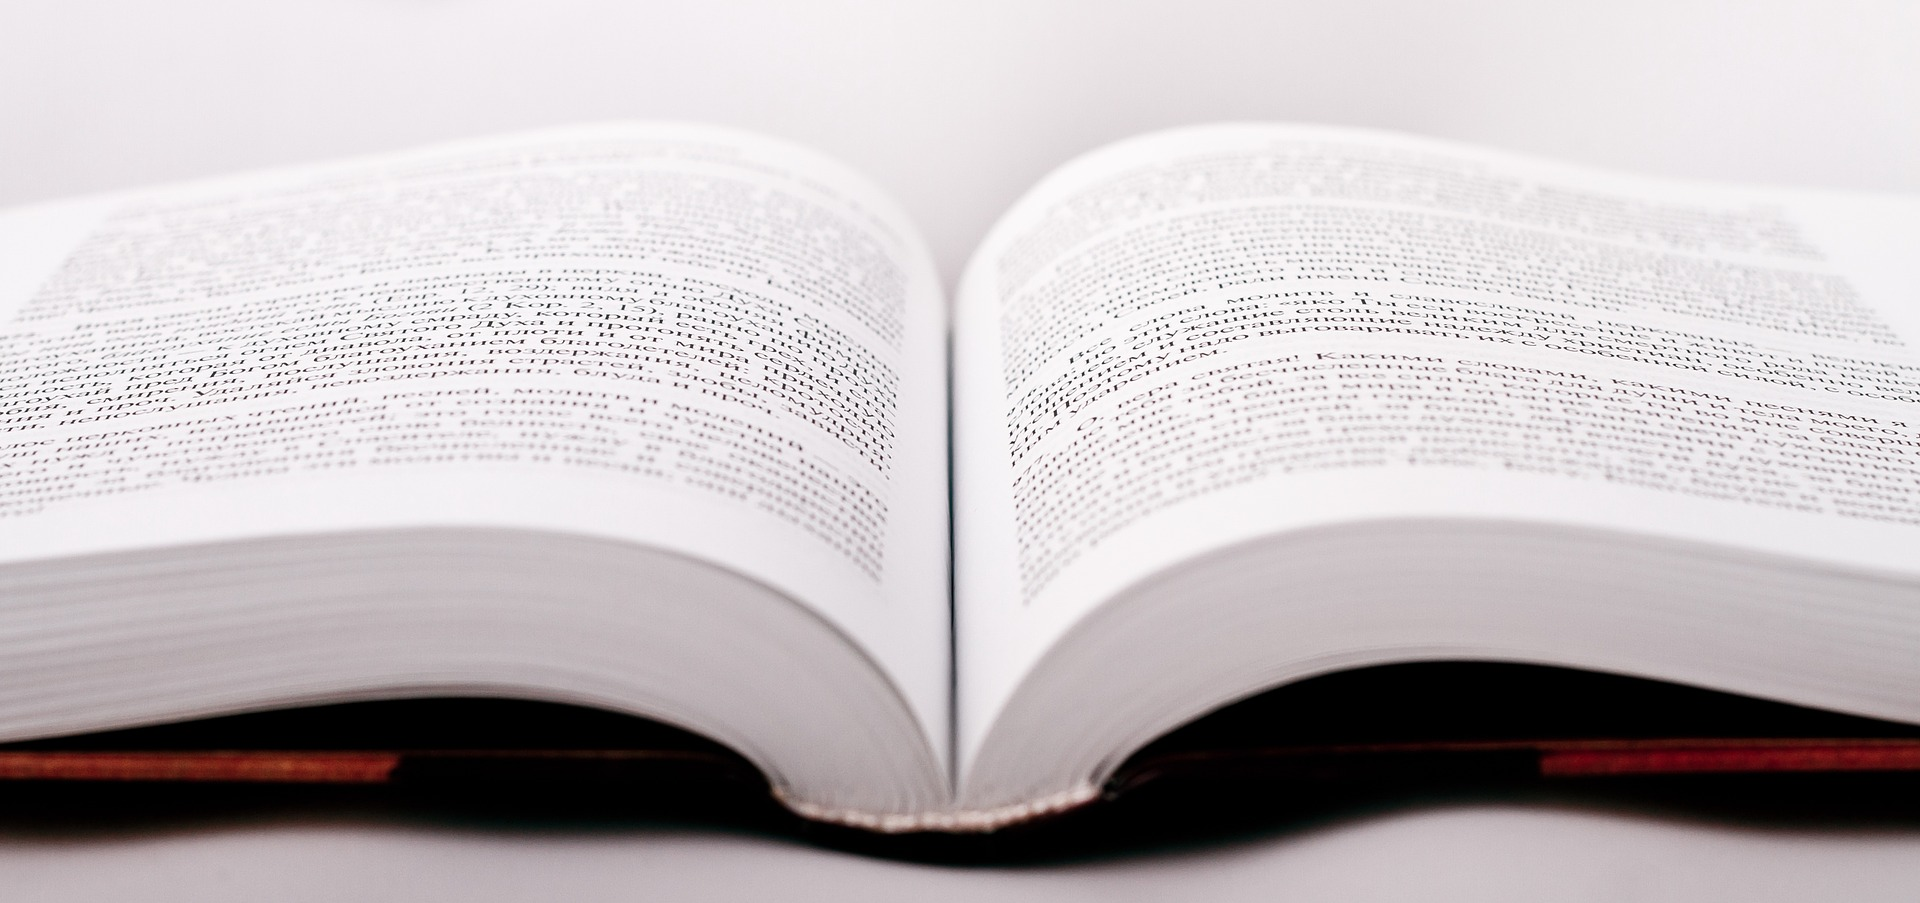
\includegraphics[width=1.5cm]{figs/bookpages}
{\small \href{https://pixabay.com/en/book-reading-library-literature-1261800/}{Libro}, por NikolayFrolochkin, Pixabay. \\ Licencia: Creative Commons CC0\\}

\end{frame}

\frame{
~
\vspace{1cm}

\begin{flushright}


\includegraphics[width=2.2cm]{figs/by-sa}
\

\begin{footnotesize}
\copyright 2022-2025 Jesus M. Gonzalez-Barahona. \\

\vspace{.4cm}

Algunos derechos reservados. Este documento se distribuye bajo los términos de la Licencia Creative Commons ``Atribución-CompartirIgual 4.0'', disponible en \\
{\scriptsize \url{http://creativecommons.org/licenses/by-sa/4.0/}} \\

\vspace{.4cm}

Este documento (incluye fuente) está disponible en \\
\url{https://jgbarah.github.io/presentations}

\end{footnotesize}
\end{flushright}

}
%%

%\againframe{firstframe}

\end{document}

%%% Local Variables:
%%% mode: latex
%%% TeX-master: t
%%% End:
